% Create a Table of Contents in Beamer
\documentclass[10pt,t]{beamer}
% Theme choice:
\usetheme{Singapore}
\useoutertheme{sidebar}
\usecolortheme{seahorse}
\setbeamercolor{titlelike}{bg=white}
\setbeamercolor{frametitle}{bg=white}
%\setbeamertemplate{frametitle}[default][left]
\setbeamertemplate{navigation symbols}{}
\setbeamertemplate{footline}{\begin{flushright}\small \insertframenumber\end{flushright}}


\usepackage{graphicx}
\usepackage{amsmath}
\usepackage{amsfonts}
\usepackage{amssymb}
\usepackage{amsthm}
\usepackage{ulem}
\usepackage{listings}

% Title page details: 
\title{Chapter 1a: Simple Linear Regression} 
\author{Nina Galanter}
\date{\today}


\begin{document}
	% Title page frame
	\begin{frame}
	\titlepage 
\end{frame}

\begin{frame}{Learning objectives}
By the end of Chapter 1a, you should be able to:
\begin{itemize}
	\item Formulate a regression model, given a scientific or statistical question
	\item Interpret the coefficients for a simple linear regression model
	\item Interpret confidence intervals and p-values for linear regression coefficients
	\item Understand the assumptions required for linear regression
	\item Use \texttt{R} to fit a simple linear regression model (and know where in the output to look for the information we need to interpret results)
	\item Create graphs to support your linear regression analysis
\end{itemize}
\end{frame}

% Outline frame
\begin{frame}{Outline}
\tableofcontents
\end{frame}

\AtBeginSection[ ]
{
\begin{frame}{Outline}
\tableofcontents[currentsection]
\end{frame}
}

% Presentation structure

\begin{frame}{Technical Content}
	
I will use this symbol next to content that is more technical. I don't expect you to know this material for the course, but I've included it as some of you might find these details helpful.
\smallskip
\begin{figure}
	\centering
	
\includegraphics[scale=0.15]{technical}
\end{figure}

\end{frame}


\section{Simple linear regression models}

\begin{frame}{MRI Dataset}
	
	We will look at another data example in this chapter:\footnote{Source: \url{https://biostat.app.vumc.org/wiki/pub/Main/CourseBios312/mri.pd}}
	\smallskip
	
	
	\begin{itemize}
	 \item In about 1986, a government sponsored cohort study of adults aged 65 years and older was conducted to observe the incidence of cardiovascular disease (especially heart attacks and congestive heart failure) and cerebrovascular disease (especially strokes) in older adults
	\medskip
	
	\item Generally healthy adults were randomly selected from Medicare rolls. Agreement to participate was high, and thus the sample can be regarded as a fairly accurate representation of healthy older Americans. 
	\medskip
	
	\item  This data includes only some of the variables and only 735 of the thousands of participants.
	
\end{itemize}


\end{frame}

\begin{frame}{MRI Data}
	
	
	Variables include:
	\smallskip	
	
	\begin{itemize}
		\item \texttt{atrophy}: A measure of global brain atrophy detected on MRI. In persons with shrinking (atrophy) of the brain, certain fluid filled cavities in the cerebrum (the ventricles) become larger. From the MRI exam, a measurement of the degree of ventricular enlargement relative to predicted ventricular size was made. These measurements were then rescaled to be a number between 0 and 100, with 0 indicating no ventricular enlargement and 100 indicating the most severe degree of atrophy
		\medskip
		
		\item \texttt{age}: Participant age at time of MRI (years)
		\medskip
		
		\item \texttt{chf} Indicator of whether the participant had been diagnosed with congestive heart failure prior to MRI (0= no, 1= yes). Congestive heart failure is a condition in which the heart muscle becomes too weak to pump blood properly.
	\end{itemize}
	


	
\end{frame}


\begin{frame}{Simple linear regression}

We can first create a scatter plot of age versus atrophy score.

\vspace{0.3cm}

\begin{figure}
	\centering \includegraphics[scale=0.6]{atrophy_age_scatter}
\end{figure}

\end{frame}

\begin{frame}{Simple linear regression}
Suppose we want to know how age and atrophy are \textit{linearly} related to each other. To do this, we need to draw a line (\textcolor{red}{$y = a + bx$}) through our data:

\vspace{0.3cm}
\begin{figure}
\centering \includegraphics[scale=0.6]{atrophy_age_scatter_badline}
\end{figure}

\end{frame}

\begin{frame}{Simple linear regression}


\begin{figure}
	\centering \includegraphics[scale=0.6]{atrophy_age_scatter_badline}
\end{figure}

\vspace{0.3cm}

This line seems bad. Can we articulate \textit{why} it seems bad? Can we articulate why it seems bad \textit{mathematically}?

\end{frame}

\begin{frame}{Simple linear regression}

\begin{figure}
	\centering \includegraphics[scale=0.6]{atrophy_age_scatter_2lines}
\end{figure}

\vspace{0.3cm}
\small This line seems better! But is it the \textit{best}? And how do we define best?

\end{frame}

\begin{frame}{Simple linear regression}
	
	
	
Simple linear regression is a statistical tool that allows us to estimate the ``best" fitting line through two variables. In general, we use linear regression with \textbf{quantitative} outcomes. Below we show our guesses for the best fitting line and the line estimated from simple linear regression in \textbf{black}:

\begin{figure}
	\centering \includegraphics[scale=0.5]{atrophy_age_scatter_bestline}
\end{figure}

\end{frame}

\begin{frame}{Simple linear regression}
	
	\vspace{-5 mm}
	
Lines take the form \textcolor{red}{$y = a + bx$}. When writing regression models we'll use the notation $E[Y \mid X] = \beta_0 + \beta_1 X$. Translating this, we have

\vspace{0.3cm}

\begin{itemize}
	\item $\beta_0$: The intercept of the linear regression line
	\item $\beta_1$: The slope of the linear regression line
	\item $E[Y]$: The average value of $Y$ in the population
	\item $E[Y \mid X]$: The average value of $Y$ in the population, given the predictor $X$ \pause
	\smallskip
	\item Examples: $Y$ is atrophy score, $X$ is whether someone has been diagnosed with congestive heart failure. The following might be true for the population of US adults over 65
	\begin{itemize}
		\smallskip
		\item $E[Y] = 35$ points (average score in the population)
		\item $E[Y \mid X = 0] = 34$ points (average score for those in the population not diagnosed with CHF)
		\item $E[Y \mid X = 1] = 40$ points (average score for those in the population diagnosed with CHF)
	\end{itemize}
\end{itemize}
\end{frame}

\begin{frame}{Simple linear regression: types of predictors}
Our example with age and atrophy score had a quantitative outcome \textit{and} a quantitative predictor. 

\vspace{0.3cm}

We can also do simple linear regression with other types of predictors, such as binary or categorical (the illustrative plots just don't look quite as nice). In HW2 you'll get the chance to explore some of this!
\end{frame}

\begin{frame}{Correlation}
When describing the linear relationship between two variables, we often talk about \textcolor{blue}{correlation}. 

\vspace{0.3cm}

\textcolor{blue}{Correlation}: The degree to which two variables are \textit{linearly} related to each other. Correlation coefficients, which we'll denote by $r$, can take values between -1 and 1:

\vspace{0.3cm} \pause
\begin{itemize}
	\item $r = -1$: perfect \textit{negative} correlation
	\item $r = 0$: no correlation
	\item $r = 1$: perfect \textit{positive} correlation
\end{itemize}

\vspace{0.3cm} \dots and any other values of $r$ in between -1 and 1 correspond to either weak or strong, negative or positive correlation.


\end{frame}

\begin{frame}{Correlation: Example}
	\centering 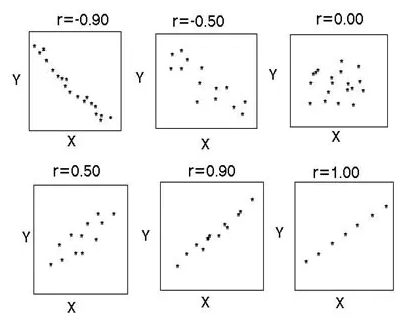
\includegraphics[scale=0.5]{correlation.png}
\end{frame}

\begin{frame}{Correlation}
Testing the null hypothesis $H_0: r = 0$ is equivalent to testing if $\beta_1$ (the slope of the simple linear regression line) is equal to zero. 



\vspace{0.3cm}

For this course, we'll focus on using correlation coefficients only as a means to describe the relationship between two variables, rather than use them to conduct hypothesis tests.

\vspace{0.3cm}


\includegraphics[scale=0.02]{technical} When we talk about correlation coefficients in this class, we are talking specifically about \textit{Pearson's} correlation coefficient. Other types of correlation coefficients exist, but Pearson's is most commonly used.
\end{frame}

\begin{frame}{\textcolor{red}{Caution!} Correlation is not Association}
	Correlation is a measure of \textbf{linear} association. The plot below shows variables which aren't correlated but are associated. Variables which are correlated are associated, but variables that are associated aren't necessarily correlated.
	
	\begin{figure}
		\centering
		\includegraphics[scale = 0.5]{quadratic_assoc}
	\end{figure}
\end{frame}



\section{Estimation \& Interpretation}


\begin{frame}{Coefficient interpretation}
The coefficients ($\beta_0, \beta_1$) in our simple linear regression model $E[Y \mid X] = \beta_0 + \beta_1 X$ often have useful interpretations.

\vspace{0.3cm} 

How do you interpret $\beta_0$ and $\beta_1$?

\vspace{0.3cm} 

\small (Hint: think about how we interpret $a$ and $b$ in $y = a + bx$)

\normalsize 
\vspace{0.3cm} 

\begin{itemize}
	\item \textcolor{blue}{$\beta_0$} 
	\item \textcolor{blue}{$\beta_1$} 
\end{itemize}

\end{frame}

\begin{frame}{Coefficient interpretation}
The coefficients ($\beta_0, \beta_1$) in our simple linear regression model $E[Y \mid X] = \beta_0 + \beta_1 X$ often have useful interpretations.

\vspace{0.3cm} 

How do you interpret $\beta_0$ and $\beta_1$?

\vspace{0.3cm} 

\small (Hint: think about how we interpret $a$ and $b$ in $y = a + bx$)
\normalsize 
\vspace{0.3cm} 

\begin{itemize}
	\item \textcolor{blue}{$\beta_0$} is the mean value of $Y$ among subjects with $X = 0$
	\item \textcolor{blue}{$\beta_1$} 
\end{itemize}

\end{frame}

\begin{frame}{Coefficient interpretation}
The coefficients ($\beta_0, \beta_1$) in our simple linear regression model $E[Y \mid X] = \beta_0 + \beta_1 X$ often have useful interpretations.

\vspace{0.3cm} 

How do you interpret $\beta_0$ and $\beta_1$?

\vspace{0.3cm} 

\small (Hint: think about how we interpret $a$ and $b$ in $y = a + bx$)

\normalsize 
\vspace{0.3cm} 

\begin{itemize}
	\item \textcolor{blue}{$\beta_0$} is the mean value of $Y$ among subjects with $X = 0$
	\item \textcolor{blue}{$\beta_1$} is the difference in mean value of $Y$ comparing two groups that differ by one unit in $X$
\end{itemize}

\end{frame}

\subsection{Slopes and Intercepts}

\begin{frame}{Interpreting slopes: mathematical explanation}
For a regression model $E[Y \mid X] = \beta_0 + \beta_1 X$, we noted that the interpretation of the slope $\beta_1$ is the difference in mean value of $Y$ comparing two groups that differ by one unit in $X$. 

\vspace{0.3cm}

Why is this the correct interpretation? Let's do some algebra\dots \pause

\vspace{0.3cm}

\begin{itemize}
	\item $E[Y \mid X = x] = \beta_0 + \beta_1 x$ \pause
	\item $E[Y \mid X = (x + 1)] = \beta_0 + \beta_1 (x + 1) = \beta_0 + \beta_1 x + \beta_1$ \pause
	\item $E[Y \mid X = (x + 1)] - E[Y \mid X = x] = \beta_1$ 
\end{itemize}

\end{frame}

\begin{frame}{Practice: interpreting intercepts in context}

Suppose we fit a linear regression model with atrophy score (0 to 100) as our outcome, and age in years as our predictor:

\begin{align*}
E[\text{atrophy} \mid \text{age}] & = -16.06 + 0.70 \times \text{age}
\end{align*}

\textcolor{purple}{Pollev:} Which of the following is the correct interpretation?
\medskip

\begin{enumerate}
	\item A person of age $0$ will have atrophy score equal to -16.06.
	\item Among all people of age $0$, the average atrophy score is -16.06.
\end{enumerate}

\medskip
\url{https://PollEv.com/multiple_choice_polls/1cLNtCZAXCZzj2Sh6evWG/respond}
\end{frame}

\begin{frame}{Practice: interpreting intercepts in context}
	
	Suppose we fit a linear regression model with atrophy score (0 to 100) as our outcome, and age in years as our predictor:
	
	\begin{align*}
	E[\text{atrophy} \mid \text{age}] & = -16.06 + 0.70 \times \text{age}
	\end{align*}
	
	\textcolor{purple}{Pollev:} Which of the following is the correct interpretation?
	\medskip
	
	\begin{enumerate}
		\item \sout{A person of age $0$ will have atrophy score equal to -16.06.}
		\item \textcolor{blue}{Among all people of age $0$, the average atrophy score is -16.06.}
	\end{enumerate}
\end{frame}

\begin{frame}{Practice: interpreting intercepts in context}


\begin{align*}
E[\text{atrophy} \mid \text{age}] & = -16.06 + 0.70 \times \text{age}
\end{align*}

Which of the following is the correct interpretation?

\vspace{0.3cm}

\begin{enumerate}
	\item[] \textcolor{blue}{Among all people of age $0$, the average atrophy score is -16.06.}
\end{enumerate}

Questions to consider when interpreting intercepts:

\begin{itemize}
	\item What is the scientific interpretation of ``a atrophy score of -16.06"? Does our intercept make scientific sense?
	\item Is our intercept within the range of our observed data (i.e. are there people age $0$ in our dataset), or would we be \textit{extrapolating} in talking about people of age $0$?
\end{itemize}

\end{frame}

\begin{frame}{Practice: interpreting slopes in context}

Suppose we fit a linear regression model with atrophy score (0 to 100) as our outcome, and age in years as our predictor:

\begin{align*}
E[\text{atrophy} \mid \text{age}] & = -16.06 + 0.70 \times \text{age}
\end{align*}


\textcolor{purple}{Pollev:} Which of the following is the correct interpretation?

\begin{enumerate}
	\item For every one year increase in age, average atrophy score increases by 0.70 points.
	\item Comparing two groups of people who differ by one year in age, the difference in average atrophy score will be 0.70 points, with the higher average score in the older of the two groups.
\end{enumerate}
\medskip

\url{https://PollEv.com/multiple_choice_polls/Llw1253pC1ll3BEMntJM3/respond}

\end{frame}

\begin{frame}{Practice: interpreting slopes in context}
	
	Suppose we fit a linear regression model with atrophy score (0 to 100) as our outcome, and age in years as our predictor:
	
	\begin{align*}
	E[\text{atrophy} \mid \text{age}] & = -16.06 + 0.70 \times \text{age}
	\end{align*}
	
	
	\textcolor{purple}{Pollev:} Which of the following is the correct interpretation?
	
	\begin{enumerate}
		\item \sout{For every one year increase in age, average atrophy score increases by 0.70 points.}
		\item \textcolor{blue}{Comparing two groups of people who differ by one year in age, the difference in average atrophy score will be 0.70 points, with the higher average score in the older of the two groups.}
	\end{enumerate}\pause

Why?
\begin{itemize}
	\item[] This was an observational study! The word ``increases" in the first interpretation implies causality, which we cannot assume in an observational study.
\end{itemize}

\end{frame}

\begin{frame}{Why do we care about the slope?}
	
	\vspace{-5 mm}
	
\textcolor{purple}{Pollev} In which example(s) is there \textbf{no} association between age and atrophy?
\url{https://PollEv.com/multiple_choice_polls/Nv7hfwA6kGK5nahuOtX8U/respond}
\vspace{0.3cm}

\begin{figure}
\centering 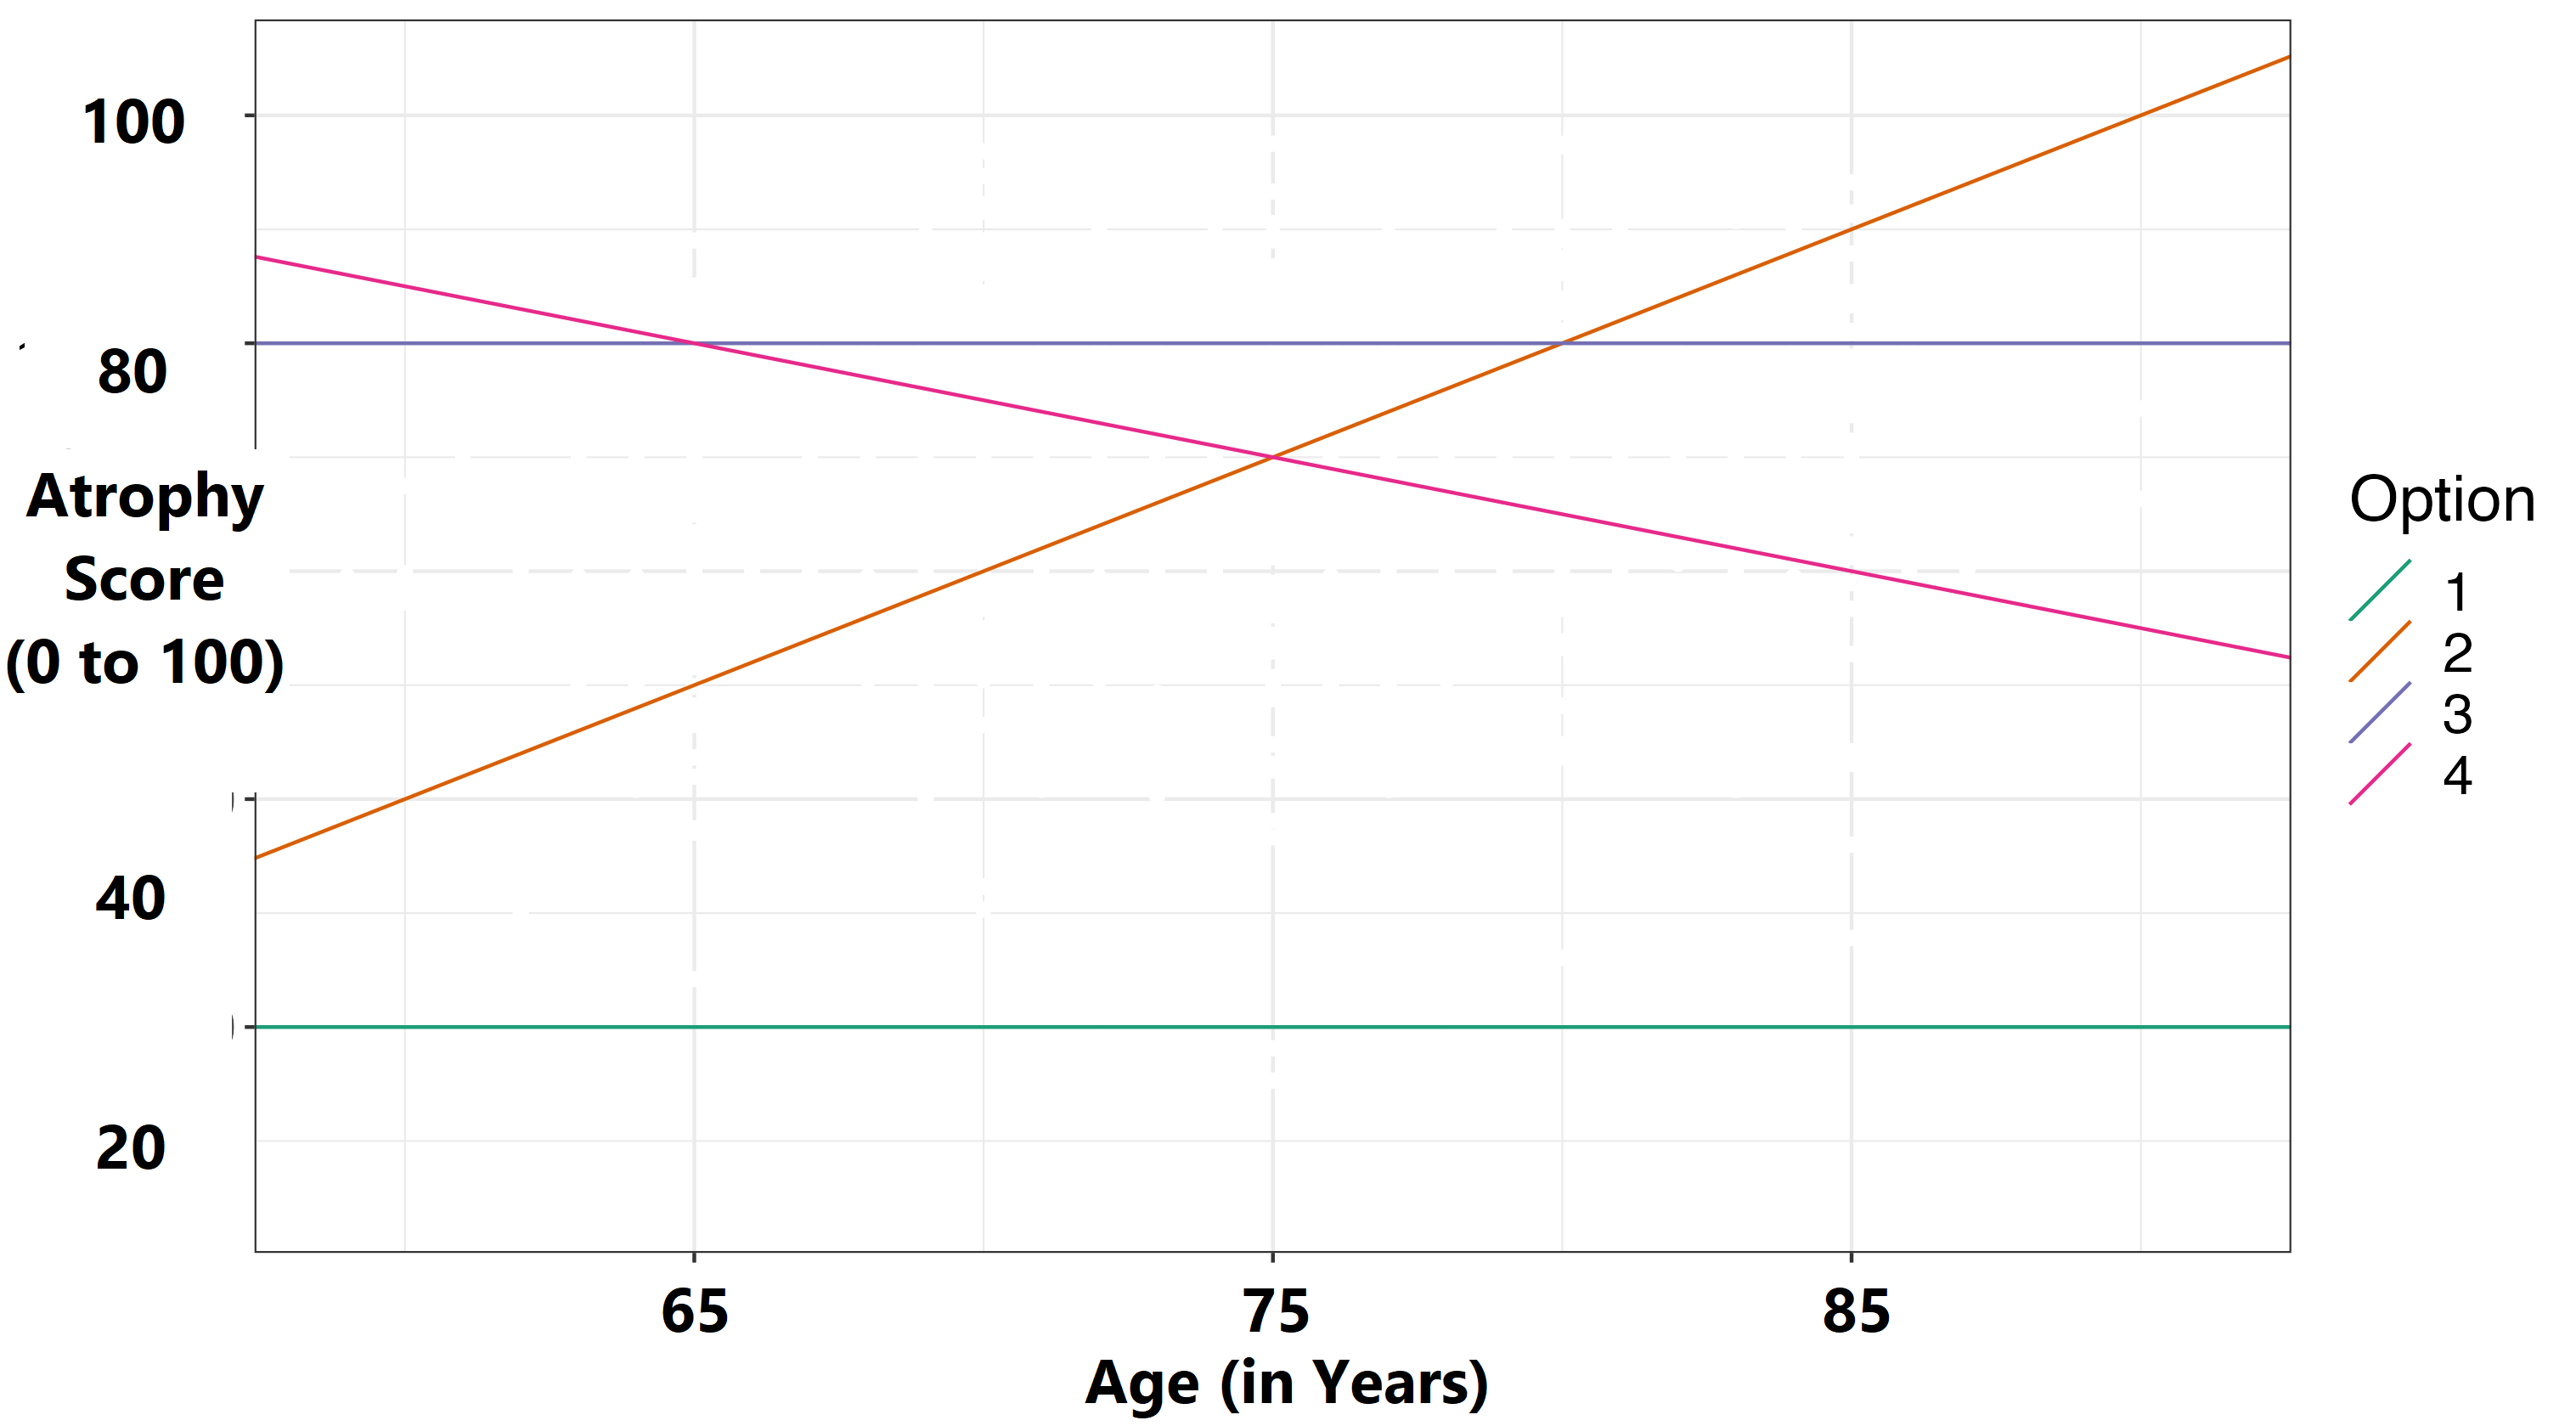
\includegraphics[scale=0.35]{zeroslopes.png}
\end{figure}\pause

\vspace{0.2cm}

\textit{What is the slope in those cases?}

\end{frame}

\begin{frame}{Why do we care about the slope?}
When
\begin{itemize}
	\item $\beta_1 = 0$: there is no linear association between $X$ and $Y$
	\item $\beta_1 > 0$: there is a positive linear association between $X$ and $Y$
	\item $\beta_1 < 0$: there is a negative linear association between $X$ and $Y$ \pause
\end{itemize}

\vspace{0.3cm}

Consider the \textbf{scientific question:} \textit{is there an association between atrophy and age?}

\vspace{0.3cm}

We can use linear regression to answer this question:

\begin{enumerate}
	\item Fit the model $E[\text{atrophy} \mid \text{age}] = \beta_0 + \beta_1 \times \text{age}$
	\item Check whether or not $\beta_1 = 0$ \textcolor{blue}{(estimate, CI, p-value)}*
\end{enumerate}

\vspace{0.3cm}

* Note: our \textbf{null hypothesis} here (that there is \textit{no} association between atrophy and age) can be written as $H_0: \beta_1 = 0$

\end{frame}

\begin{frame}{Why do we care about the slope?}
When
\begin{itemize}
	\item $\beta_1 = 0$: there is no linear association between $X$ and $Y$
	\item $\beta_1 > 0$: there is a positive linear association between $X$ and $Y$
	\item $\beta_1 < 0$: there is a negative linear association between $X$ and $Y$
\end{itemize}

\vspace{0.3cm}

Consider the \textbf{scientific question:} \textit{is there an association between atrophy and age?}

\vspace{0.3cm}

We can use linear regression to answer this question:

\begin{enumerate}
	\item Fit the model $E[\text{atrophy} \mid \text{age}] = \beta_0 + \beta_1 \times \text{age}$
	\item Check whether or not $\beta_1 = 0$ \textcolor{blue}{(estimate, CI, p-value)}
\end{enumerate}

\vspace{0.3cm}

What \textbf{statistical question} are we answering? \textit{Is there an association between atrophy and age, where association is quantified by the difference in mean atrophy between age groups}

\end{frame}

\subsection{Hypothesis tests}

\begin{frame}{Hypothesis tests}
Consider the regression model:
$$
E[Y \mid X] = \beta_0 + \beta_1 X
$$
We know that $\beta_1$ quantifies the association between $X$ and $Y$.

\vspace{0.3cm}

To test whether there is a \textit{statistically significant} association between $X$ and $Y$, \textcolor{blue}{we need to test whether $\beta_1 = 0$:}

\begin{itemize}
	\item $H_0: \beta_1 = 0$
	\item $H_1: \beta_1 \neq 0$
\end{itemize} \pause

\vspace{0.3cm}

Interpret the $p$-value as we have before in Chapter 0:
\begin{itemize}
	\item $p < \alpha$: \textbf{reject} $H_0$, ``we have evidence to suggest that $X$ is associated with $Y$"
	\item $p > \alpha$: \textbf{fail to reject} $H_0$, ``we do not have enough evidence to support the hypothesis that $X$ is associated with $Y$"
\end{itemize}

\end{frame}

\subsection{Uncertainty}

\begin{frame}{Standard errors (SEs) and confidence intervals}
When we estimate regression coefficients, we also want to quantify the \textit{uncertainty} in these estimates. Once we have our standard error, we can calculate a 95\% confidence interval.


\end{frame}

\begin{frame}{Standard errors (SEs) and confidence intervals}

We have two options for 95\% confidence intervals:
\begin{enumerate}
	\item $\hat{\beta} \pm 1.96 \times \hat{SE}(\hat{\beta})$
	\item $\hat{\beta} \pm t_{n-2} \times \hat{SE}(\hat{\beta})$
	\begin{itemize}
		\item If $n = 10$, $t_{n-2} = 2.31$
		\item If $n = 100$, $t_{n-2} = 1.98$
		\item If $n = 1000$, $t_{n-2} = 1.96$
	\end{itemize}
\end{enumerate}

\small (\textit{Recall that the $t$-distribution is defined by its \textit{degrees of freedom}, which is $n-2$ in the case of simple linear regression with a single predictor})

\vspace{0.3cm}

\normalsize The first option is what we are used to seeing. The latter is what is commonly provided in statistical software. The key takeaway for this course is that \textbf{when n} (our sample size) \textbf{is large}, there is little difference between the confidence intervals from options 1 and 2, and the interpretation of the confidence interval remains the same. If you'd like more details on why statistical software typically provides confidence intervals based on a $t$-distribution, please come ask in office hours!

\end{frame}

\begin{frame}{Interpreting 95\% confidence intervals}
Returning to our example of using linear regression to assess the association between atrophy and age, suppose we estimate the slope to be 0.70, with a 95\% confidence interval (0.53, 0.86).

\vspace{0.3cm}

Slope interpretation:

\vspace{0.3cm}

\textit{Comparing two groups of people who differ by one year in age, the difference in average atrophy will be 0.70 points, with the higher average atrophy in the older of the two groups.}

\vspace{0.3cm}

How would we interpret the confidence interval for this slope estimate? % have them chat with a partner

\end{frame}

\begin{frame}{Interpreting 95\% confidence intervals}
Returning to our example of using linear regression to assess the association between atrophy and age, suppose we estimate the slope to be 0.70, with a 95\% confidence interval (0.53, 0.86).

\vspace{0.3cm}

Confidence interval interpretation:

\vspace{0.3cm}

\textit{Comparing two groups of people who differ by one year in age, the difference in average atrophy will be 0.70 points, with the higher average atrophy in the older of the two groups. \textcolor{blue}{Based on a 95\% confidence interval, this estimated difference would not be judged unusual if the true difference were between 0.53 and 0.86 points.}}

\vspace{0.3cm}

\small Note that this is the same language as the confidence interval interpretation for a mean or difference in means, as in Chapter 0!

\end{frame}

\begin{frame}{Connection between confidence intervals and $p$-values}
	
\textcolor{purple}{Pollev:} Suppose we have access to the estimate of the slope (0.70) and a 95\% confidence interval to go with it (0.53, 0.86), as before, where our null hypothesis was that the slope was $0$. What can we say about the $p$-value for this hypothesis test?

\vspace{0.3cm}

\begin{enumerate}
	\item $p < 0.05$
	\item $p = 0.05$
	\item $p > 0.05$
	\item $p < 0.95$
\end{enumerate}
\medskip

\url{https://PollEv.com/multiple_choice_polls/zTxQPnNjYWAJ46I9PGs6D/respond}


\end{frame}

\begin{frame}{Connection between confidence intervals and $p$-values}
\textcolor{purple}{Pollev:} Suppose we have access to the estimate of the slope (0.70) and a 95\% confidence interval to go with it (0.53, 0.86), as before, where our null hypothesis was that the slope was $0$. What can we say about the $p$-value for this hypothesis test?

\vspace{0.3cm}

\begin{enumerate}
	\item \textcolor{blue}{$p < 0.05$}
	\item \sout{$p = 0.05$}
	\item \sout{$p > 0.05$}
	\item \sout{$p < 0.95$}
\end{enumerate}

\vspace{0.3cm}

The 95\% confidence interval does not contain the null hypothesis of $0$, so we reject the null hypothesis. We know that we reject $H_0$ if the p-value is smaller than some pre-specified threshold $\alpha$, which in this case is $1 - 0.95 = 0.05$ since we have a 95\% confidence interval.

\end{frame}



\begin{frame}{Putting it all together \dots}
We've now completed a linear regression ``recipe." After translating a scientific question into a statistical one, the ingredients include:

\vspace{0.3cm}

\begin{itemize}
	\item Determine the \textbf{hypotheses}: $H_0$, $H_1$
	\item Obtain an \textbf{estimate/statistic}: estimated regression coefficient
	\item \textbf{Quantify uncertainty}: 95\% confidence interval for regression coefficient
	\item Perform a \textbf{hypothesis test}: reject, or fail to reject, the null hypothesis based on p-value for regression coefficient
\end{itemize}
\end{frame}

\subsection{Examples}

\begin{frame}{Example: atrophy and age}
\begin{enumerate}
	\item \textbf{Scientific question:} is there an \textcolor{orange}{association} between brain atrophy as shown by an MRI and age?
	\item \textbf{Statistical question:} is there a \textcolor{orange}{difference in average} atrophy comparing groups of people that differ in age? \pause
	\begin{itemize}
		\item \textbf{Population:} all people in the US over the age of 65
		\item \textbf{Parameter:} population linear regression slope (diff. in means comparing groups that differ by one year in age) \pause
	\end{itemize}
	\item Take a \textbf{sample} from the population: 735 people over the age of 65 in generally good health \pause
	\item Perform \textit{statistical inference}:
	\begin{itemize}
		\item Calculate the corresponding \textbf{statistic}: sample linear regression slope (estimated diff. in means comparing groups that differ by one year in age)\pause
		\item Quantify the uncertainty in your statistic
		\item Perform a hypothesis text
	\end{itemize} \pause
	\item Make conclusions in context of original question
\end{enumerate}
\end{frame}

\begin{frame}{Example: atrophy and age}
To fit the regression model $E[\text{atrophy} \mid \text{age}] = \beta_0 + \beta_1 \times \text{age}$ in \texttt{R} we use the \texttt{lm} function, and the \texttt{confint} function to get confidence intervals (you'll get more practice with this in the HW and discussion section):

\vspace{0.15cm}

\centering 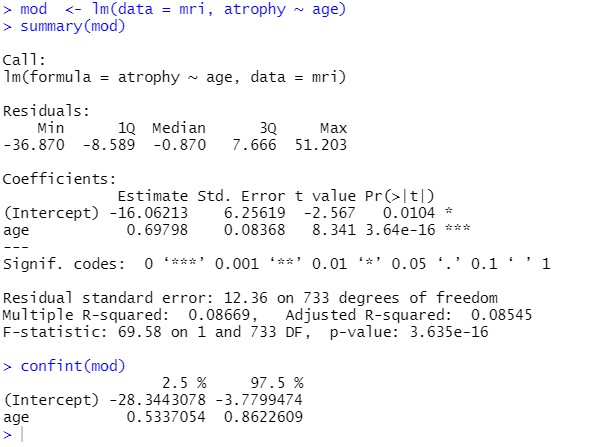
\includegraphics[scale=0.45]{atrophy_age_code}

\end{frame}

\begin{frame}{Example: atrophy and age}
The necessary pieces we need to extract from this output are (1) the estimate/statistic, (2) the p-value, and (3) the 95\% confidence interval:

\vspace{0.15cm}

\centering 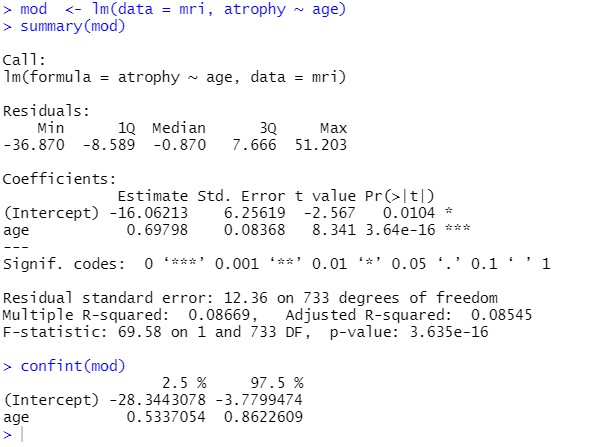
\includegraphics[scale=0.45]{atrophy_age_code}

\end{frame}

\begin{frame}{Example: atrophy and age}
Interpreting our results:
\begin{itemize}
	\item \textit{Statistic}: We estimate that the difference in mean atrophy comparing two groups of people that differ by one year in age is 0.70 points, with heigher average atrophy in the older of the two groups. \pause
	\item \textit{Uncertainty}: Based on a 95\% confidence interval, this estimated difference would not be judged unusual if the true difference were between 0.53 and 0.86. \pause
	\item \textit{Hypothesis test / p-value}: These data provide strong evidence that the difference in mean atrophy between groups of people that differ by one year in age is significantly different from zero (p $<$ 0.001). \pause
	\item \textit{Conclusion}: These data provide evidence to suggest that, among those over the age of 65, older people tend to have higher brain atrophy as detected by an MRI.
\end{itemize}
\end{frame}

\begin{frame}{Example: atrophy and age}
\textit{Why haven't we said anything about the intercept?}
\vspace{0.3cm}
\begin{itemize}
	\item Interpretation: We estimate that the average atrophy score among people of age $0$ is -16.06\pause
	\item But\dots 
	\begin{itemize}
		\item \textit{Is this scientifically relevant?} No, the study was only looking at people over the age of 65
		\item Most importantly, \textcolor{blue}{the intercept has nothing to do with our scientific question} (is atrophy score associated with age)
	\end{itemize} \pause
	\item Since the intercept is not relevant to our primary scientific question, we don't care about the CI or p-value\pause
	\item \textit{Would we ever care about the intercept?} If the intercept answers your scientific question (rare) and is relevant (sometimes, see HW), then yes!
\end{itemize}
\end{frame}

\begin{frame}{Example: birthweight and First Steps participation}
In Chapter 0 we considered the following set of questions:

\vspace{0.3cm}

\begin{enumerate}
	\item \textbf{Scientific question:} do birth parents in King County who participated in First Steps (FS) have different birth outcomes than those not in the program?
	\item \textbf{Statistical question:} is there a difference in average birthweight between birth parents in FS and those not in the program?
\end{enumerate}

\vspace{0.3cm} We previously used a two-sample t-test to address this question, but we can also use linear regression!

\end{frame}

\begin{frame}{Example: birthweight and First Steps participation}
We fit the regression model $E[\text{bwt} \mid \text{FS}] = \beta_0 + \beta_1 \times \text{FS}$ in \texttt{R} using the \texttt{lm} function, and the \texttt{confint} function to get confidence interval\dots

\vspace{0.2cm}

\centering 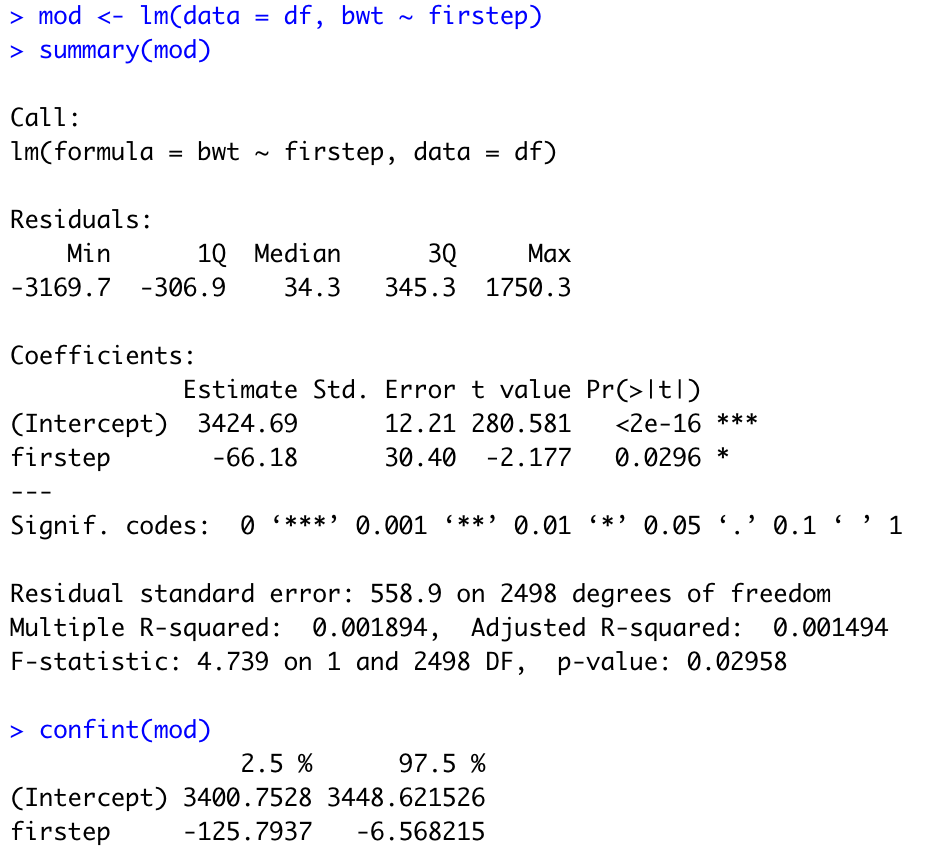
\includegraphics[scale=0.35]{lm_bwt_fs.png}
\end{frame}

\begin{frame}{Example: birthweight and First Steps participation}
\dots and we extract the necessary information from the output\dots

\vspace{0.2cm}

\centering 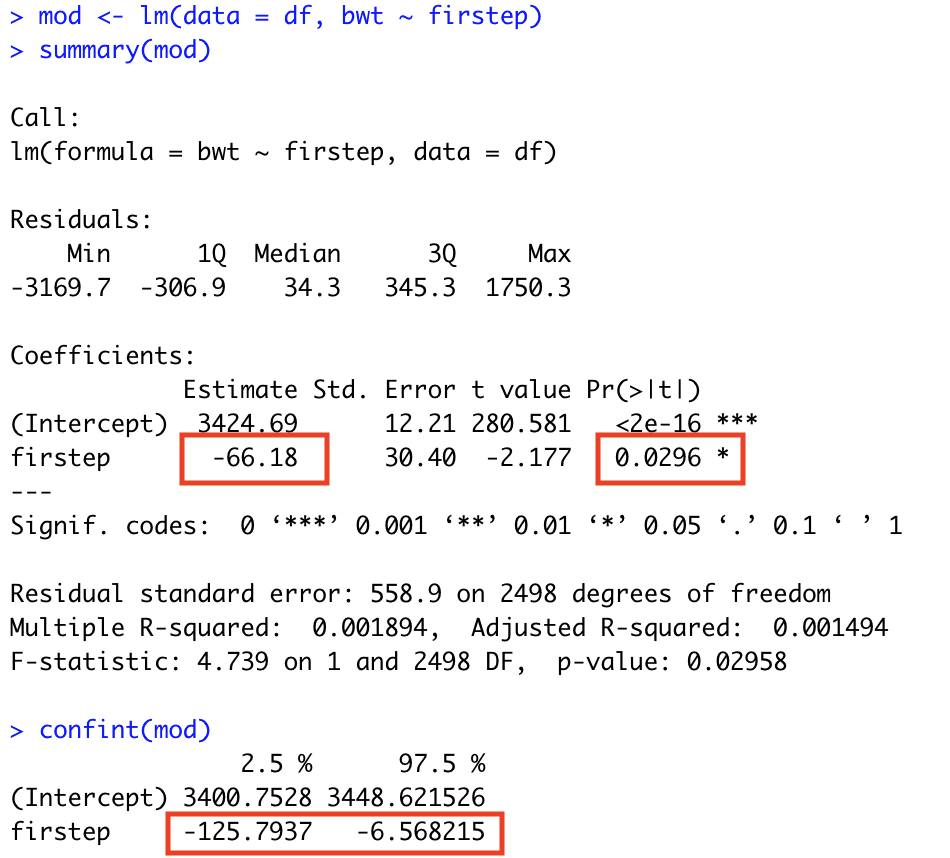
\includegraphics[scale=0.35]{lm_bwt_fs2.png}
\end{frame}

\begin{frame}{Example: birthweight and First Steps participation}
Our linear regression results:

\vspace{0.3cm}

\begin{itemize}
	\item \textit{Statistic}: We estimate the difference in mean birthweight between babies born to parents in FS vs. those not is 66.18 grams (with those in FS tending to have the lower mean birthweight). \pause
	\item \textit{Uncertainty}: Based on a 95\% confidence interval, this observed difference would not be judged unusual if the true difference were between 6.57 and 125.79 grams. \pause
	\item \textit{Hypothesis test / p-value}: These data provide strong evidence to suggest the difference in mean birthweight between groups is different from zero (p $<$ 0.05). \pause
	\item \textit{Conclusion}: These data provide evidence to suggest that babies born to birth parents in FS tend to have lower birthweights.
\end{itemize}
\end{frame}

\begin{frame}{Example: birthweight and First Steps participation}
Comparing our linear regression results to our t-test results from Chapter 0:

\vspace{0.3cm}

\begin{table}[]
	\begin{tabular}{l|ll}
		& Linear regression & T-test         \\ \hline
		Estimate & 66.18             & 66.18          \\ \hline
		95\% CI  & (6.57, 125.79)    & (1.95, 130.4) \\ \hline
		p-value  & 0.0296            & 0.043        
	\end{tabular}
\end{table} 
\medskip
Why are they different?\pause

\vspace{0.3cm}

The difference has to do with regression assumptions, which we will talk about soon!

\end{frame}

\subsection{Least squares}

\begin{frame}{Least squares estimation}
What is \texttt{R} doing \textit{under the hood} to get these regression coefficient estimates? \pause

\vspace{0.3cm}

\centering 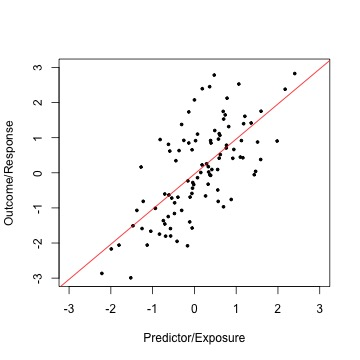
\includegraphics[scale=0.45]{linear-regr.jpg}
\end{frame}

\begin{frame}{Least squares estimation}
\textit{Least squares}: minimize the sum of the squared distances from the observed points to the fitted line

\vspace{0.3cm}

\centering 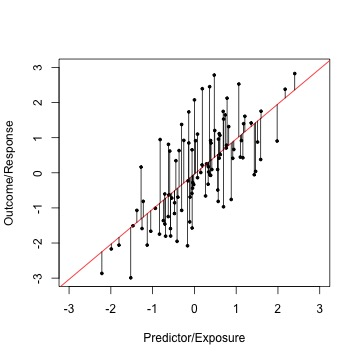
\includegraphics[scale=0.45]{linear-regr-ls.jpg}

\end{frame}

\begin{frame}{Least squares estimation: technical details 
\includegraphics[scale=0.02]{technical}}
\textit{Least squares}: minimize the sum of the squared distances from the observed points to the fitted line

\vspace{0.3cm}

Breaking this down\dots

\vspace{0.3cm}

\begin{itemize}
	\item The distance from an observed point for an individual $i$ to the fitted line is $Y_i - [\beta_0 + \beta_1 X_i]$
	\item Squaring the distance we get $(Y_i - [\beta_0 + \beta_1 X_i])^2$
	\item Summing the squared distances over all observations we get $\sum_{i = 1}^n (Y_i - [\beta_0 + \beta_1 X_i])^2$
	\item Minimizing we get $$\underset{\beta_0, \beta_1}{\text{argmin}} \sum_{i = 1}^n (Y_i - [\beta_0 + \beta_1 X_i])^2$$
\end{itemize}

\vspace{0.3cm}

\small This has a closed form solution given by $\hat{\beta}_0 =  \bar{Y} - \hat{\beta}_1 \bar{X}$, $\hat{\beta}_1 = \frac{\sum_i (X_i - \bar{X}) (Y_i - \bar{Y})}{\sum_i (X_i - \bar{X})^2}$

\end{frame}

%
%
%\section{Assumptions \& diagnostics}
%
%\begin{frame}{Linear regression form}
%We've hinted at a few necessary assumptions for linear regression, but now we spell them out in detail. So far we've been writing our regression as
%$$
%E[Y \mid X] = \beta_0 + \beta_1 X
%$$
%When we have multiple observations, it is common to label them as $i = 1, \dots, n$, where $n$ is the total number of observations in our data. Then we can write
%$$
%E[Y_i \mid X_i] = \beta_0 + \beta_1 X_i
%$$
%for each individual $i$. 
%\end{frame}
%
%\begin{frame}{Linear regression form}
%Note that so far, we've always seen the conditional expectation of $Y$ given $X$ on the left hand side of our regression equation. Instead of writing it this way, it is common to instead write,
%$$
%Y_i = \beta_0 + \beta_1 X_i + \epsilon_i
%$$
%where $\epsilon_i$ are error terms with mean zero, for each individual. 
%
%\vspace{0.3cm}
%
%To recap, we can write linear regression models in two equivalent ways:
%\begin{enumerate}
%	\item $E[Y_i \mid X_i] = \beta_0 + \beta_1 X_i$ for $i = 1, \dots, n$
%	\item $Y_i = \beta_0 + \beta_1 X_i + \epsilon_i$ for $i = 1, \dots, n$, with $E[\epsilon_i] = 0$ for all $i$
%\end{enumerate}
%
%\end{frame}
%
%
%
%\begin{frame}{Linear regression assumptions}
%We can write the \textit{classical} linear regression assumptions under the following model as follows:
%
%$$
%Y_i = \beta_0 + \beta_1 X_i + \epsilon_i \text{ for } i = 1, \dots n
%$$
%
%\begin{itemize}
%	\item \textcolor{red}{L}inearity: There is a linear relationship between $X_i$ and the true population conditional mean $Y_i \mid X_i$
%	\begin{itemize}
%		\item i.e. $E[Y_i \mid X_i] = \beta_0 + \beta_1 X_i$
%	\end{itemize}
%	\item \textcolor{red}{I}ndependence: The errors $\epsilon_i$ are independent of each other
%	\item \textcolor{red}{N}ormality: $\epsilon_i$ are normally distributed
%	\item \textcolor{red}{E}qual variance: $\epsilon_i$ have the same variance
%	\begin{itemize}
%		\item $\epsilon_i \sim N(0, \sigma^2)$, where $\sigma^2$ does not depend on $i$
%	\end{itemize}
%\end{itemize}
%
%\vspace{0.3cm}
%
%These are commonly called the \textcolor{red}{LINE} assumptions, which should hopefully make them easier to remember!
%\end{frame}
%
%\begin{frame}{Linear regression assumptions}
%We can write the \textit{classical} linear regression assumptions under the following model as follows:
%
%$$
%Y_i = \beta_0 + \beta_1 X_i + \epsilon_i \text{ for } i = 1, \dots n
%$$
%
%\begin{itemize}
%	\item \textcolor{red}{L}inearity: There is a linear relationship between $X_i$ and the true population conditional mean $Y_i \mid X_i$
%	\begin{itemize}
%		\item i.e. $E[Y_i \mid X_i] = \beta_0 + \beta_1 X_i$
%	\end{itemize}
%	\item \textcolor{red}{I}ndependence: The errors $\epsilon_i$ are independent of each other
%	\item \textcolor{red}{N}ormality: $\epsilon_i$ are normally distributed
%	\item \textcolor{red}{E}qual variance: $\epsilon_i$ have the same variance
%	\begin{itemize}
%		\item $\epsilon_i \sim N(0, \sigma^2)$, where $\sigma^2$ does not depend on $i$
%	\end{itemize}
%\end{itemize}
%
%\vspace{0.3cm}
%
%We will come back to the \textcolor{blue}{normality} and \textcolor{blue}{equal variance} assumptions shortly, because (as we'll find out) we may not actually need them!
%\end{frame}
%
%\subsection{Linearity}
%
%\begin{frame}{Linearity assumption}
%\textcolor{blue}{Linearity assumption}: The true population conditional mean is a linear function of the predictor, i.e. $E[Y \mid X] = \beta_0 + \beta_1 X$
%
%\vspace{0.3cm}
%
%What does it \textit{mean} for this assumption to be violated?
%
%\vspace{0.3cm}
%
%\begin{itemize}
%	\item[] Violating the linearity assumption means that we have incorrectly specified our \textit{mean model} (so called because we're modeling the conditional mean as a linear function of predictor(s)). For simple linear regression, this is relatively straightforward: it means that the true population conditional mean is \textit{not} a linear function of the predictor.
%\end{itemize}
%
%\vspace{0.3cm}
%
% \textcolor{blue}{We will revisit this assumption for multiple linear regression, and discuss ways in which we could incorrectly specify the mean model in that case later!}
%
%\end{frame}
%
%\begin{frame}{Linearity assumption: violations}
%
%What could a nonlinear assocation between $X$ and $Y$ look like? Lots of things! But here's an example\dots
%
%\vspace{0.3cm}
%
%\centering 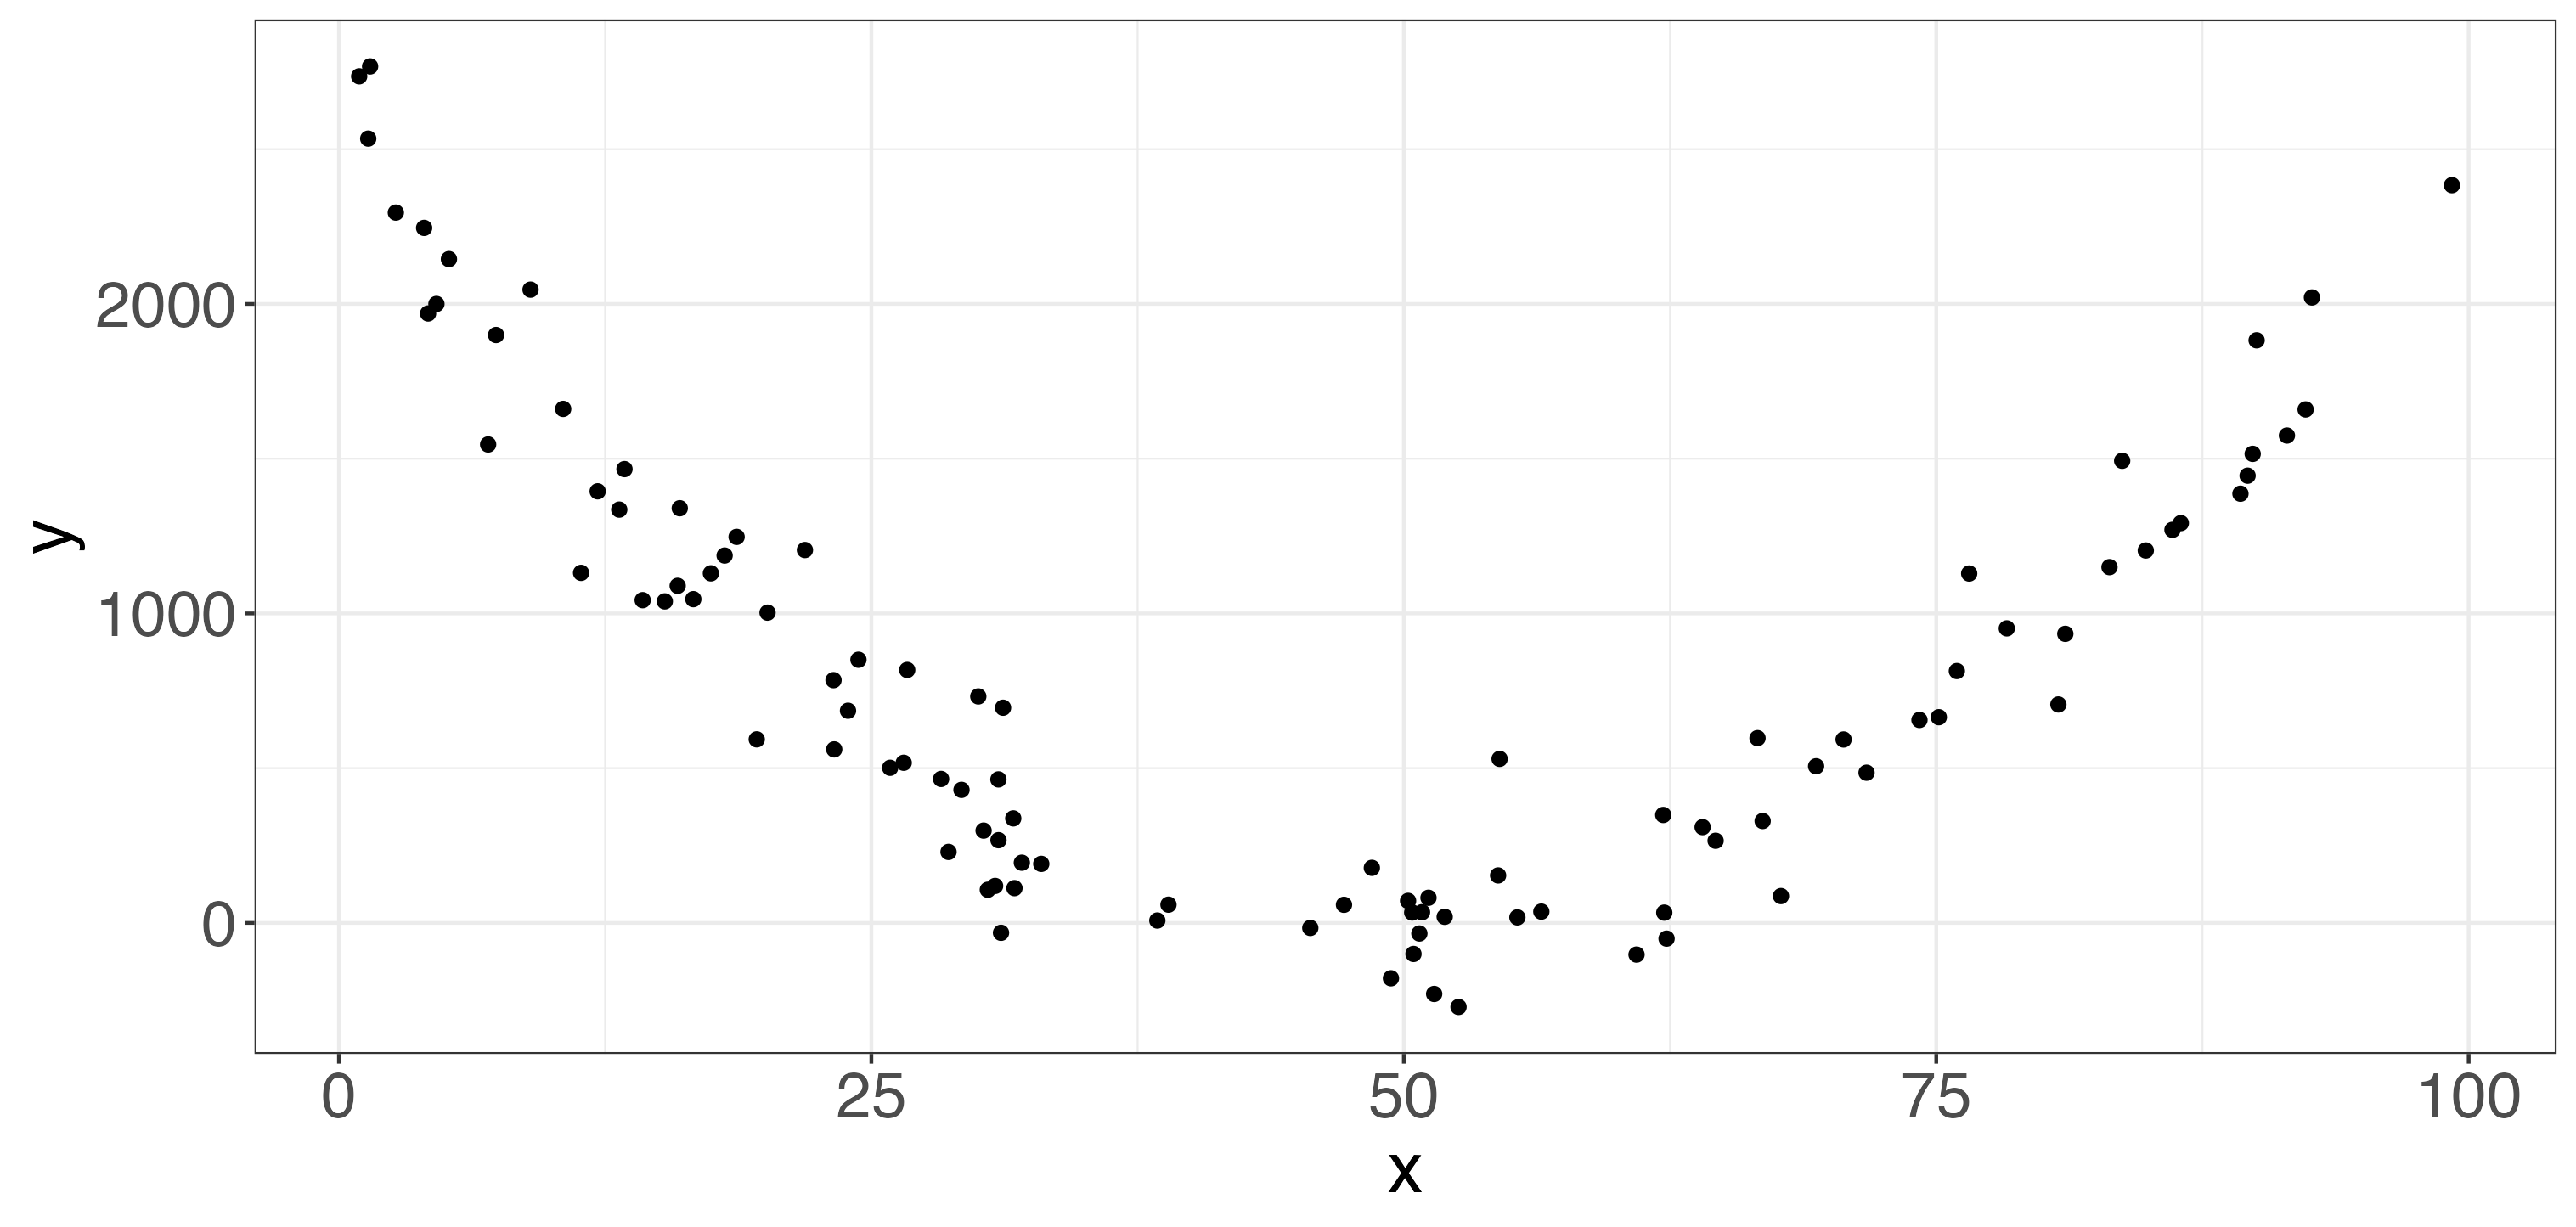
\includegraphics[scale=0.4]{quadratic.png}
%
%\end{frame}
%
%\begin{frame}{Linearity assumption: violations}
%
%\dots and here's a \textit{real world} example of the nonlinear relationship between age and mortality (commonly referred to as the Nike swoosh in demography):
%
%\vspace{0.3cm}
%
%\centering 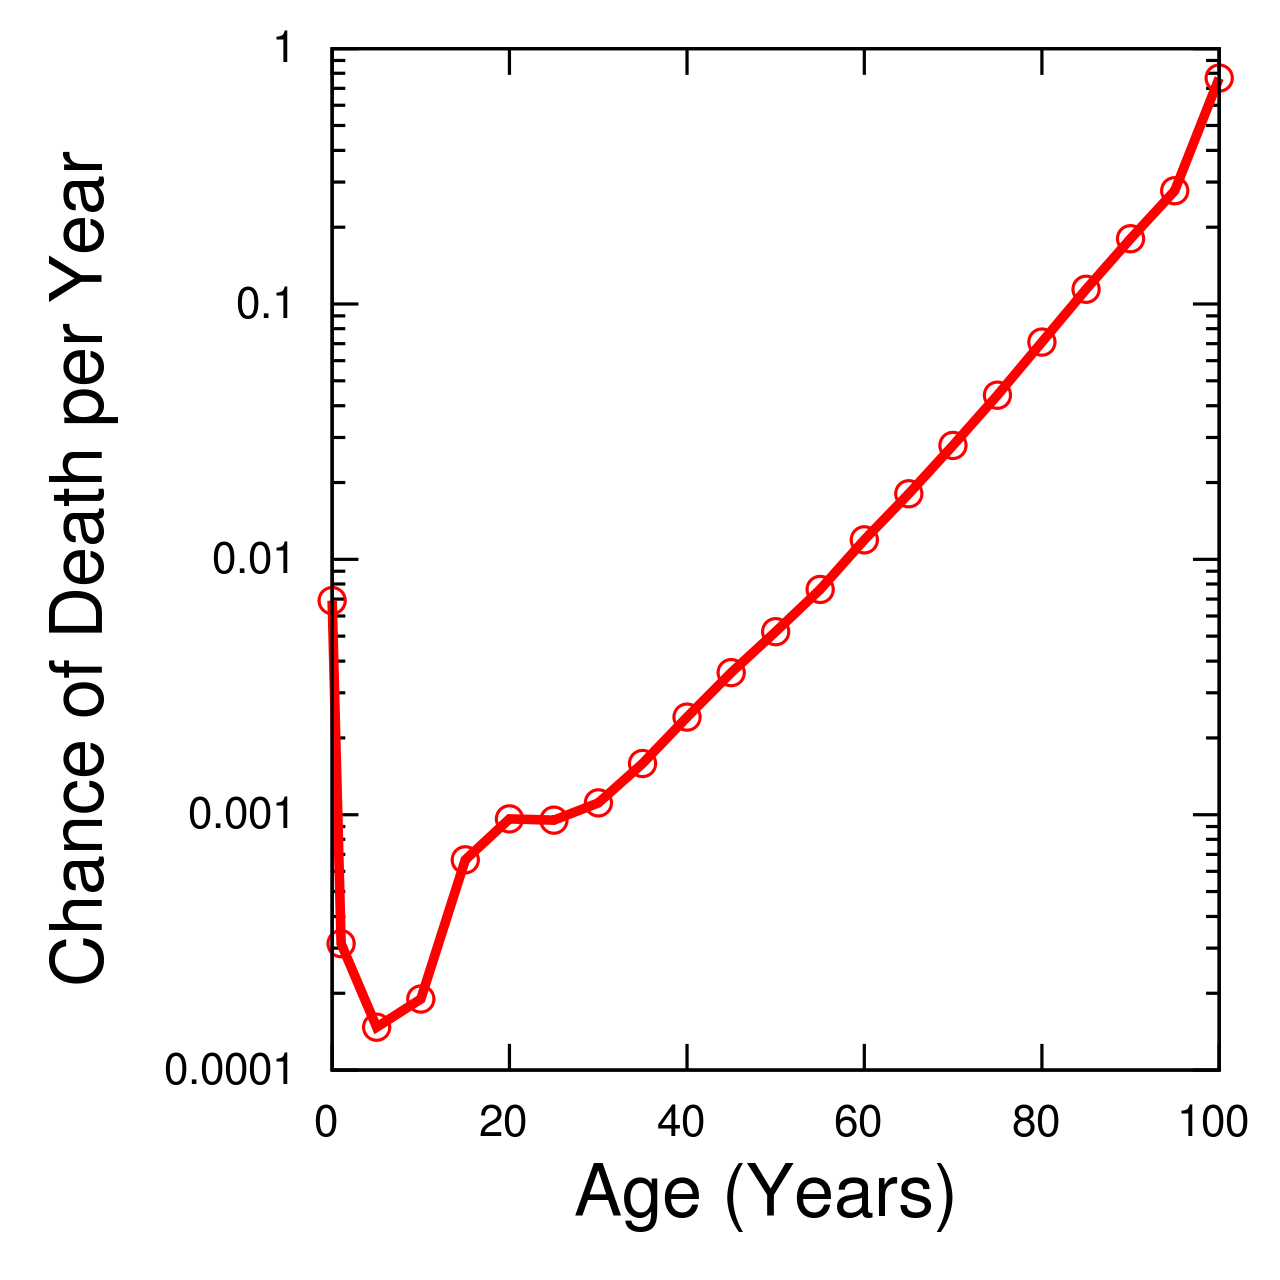
\includegraphics[scale=0.1]{mortality_curve.png}
%
%\end{frame}
%
%\begin{frame}{Linearity assumption: diagnostics}
%How do we assess whether or not the linearity assumption is violated?
%
%\vspace{0.3cm}
%
%We can plot \textcolor{blue}{residuals} vs. \textcolor{blue}{fitted values} using our linear regression output, and diagnose the assumption based on a scatter plot comparing the two.
%
%\vspace{0.3cm}
%
%\begin{itemize}
%	\item A \textcolor{blue}{fitted value} is the value of the response predicted from your regression, $\hat{\beta}_0 + \hat{\beta}_1 X$
%	\item A \textcolor{blue}{residual} is the difference between the observed value of the response variable $Y$ and the fitted value
%	\begin{itemize}
%		\item[] Residuals are our best guess at what the error terms $\epsilon_i$ for our model may look like, which is why we use them for diagnostic plots!
%	\end{itemize}
%\end{itemize}
%\end{frame}
%
%\begin{frame}[fragile]{Linearity assumption: diagnostics in \texttt{R}}
%To plot residuals vs. fitted values in \texttt{R}, we can use the following code for a given linear model object \texttt{mod}:
%
%\vspace{0.2cm}
%
%\begin{lstlisting}
%resids <- residuals(mod)
%fittedvals <- predict(mod)
%data.frame(resids = resids,
%           fittedvals = fittedvals) %>%
%	ggplot(aes(fittedvals, resids)) +
%	geom_point() +
%	geom_hline(yintercept = 0, col = "red") 
%\end{lstlisting}
%
%% \centering 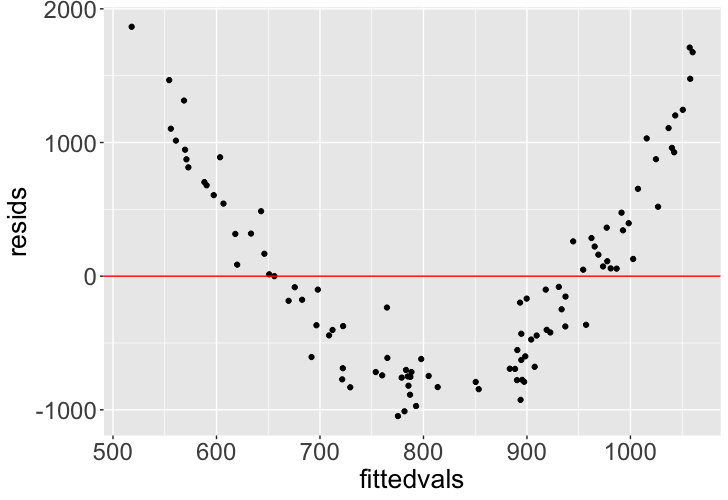
\includegraphics[scale=0.4]{fitted_resids.png}
%
%\end{frame}
%
%\begin{frame}{Linearity assumption: diagnostics in \texttt{R}}
%And we get a plot (for our example of a nonlinear association) that looks like this:
%
%\centering 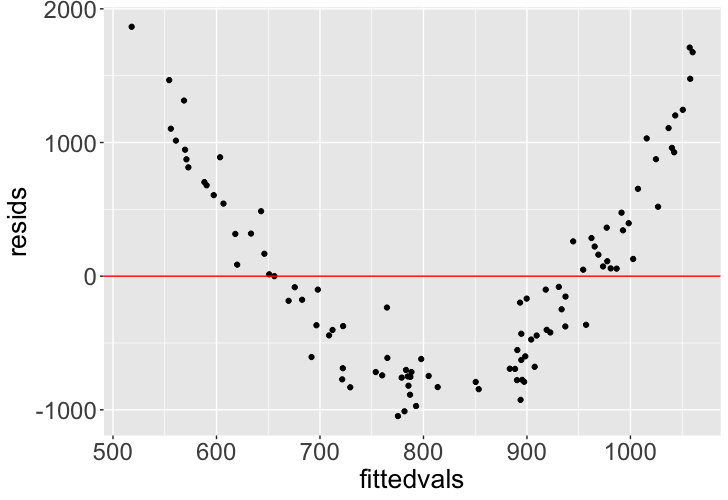
\includegraphics[scale=0.3]{fitted_resids.png}
%
%\end{frame}
%
%\begin{frame}{Linearity assumption: diagnostics in \texttt{R}}
%In this plot, what are we looking for?
%
%\vspace{0.3cm}
%
%If the linearity assumption is \textit{not} violated, then we expect there to be no clear pattern between the residuals and fitted values. If this is the case, we can roughly draw a straight line through the points at the y intercept (at $y = 0$), the red line in the plot on the previous slide. 
%
%\vspace{0.3cm}
%
%\textcolor{blue}{Question:} Do you think the linearity assumption is violated for the example on the previous slide?\pause
%
%\vspace{0.3cm}
%
%\textcolor{blue}{Answer:} The linearity assumption is violated because the residuals do not fall roughly in a straight line at the y intercept (not even close!)
%
%\end{frame}
%
%
%\begin{frame}{Linearity assumption: diagnostics}
%\textcolor{blue}{Question:} Do you think the linearity assumption is violated for models $1$ through $4$, based on the plots of fitted values vs. residuals?
%
%\centering 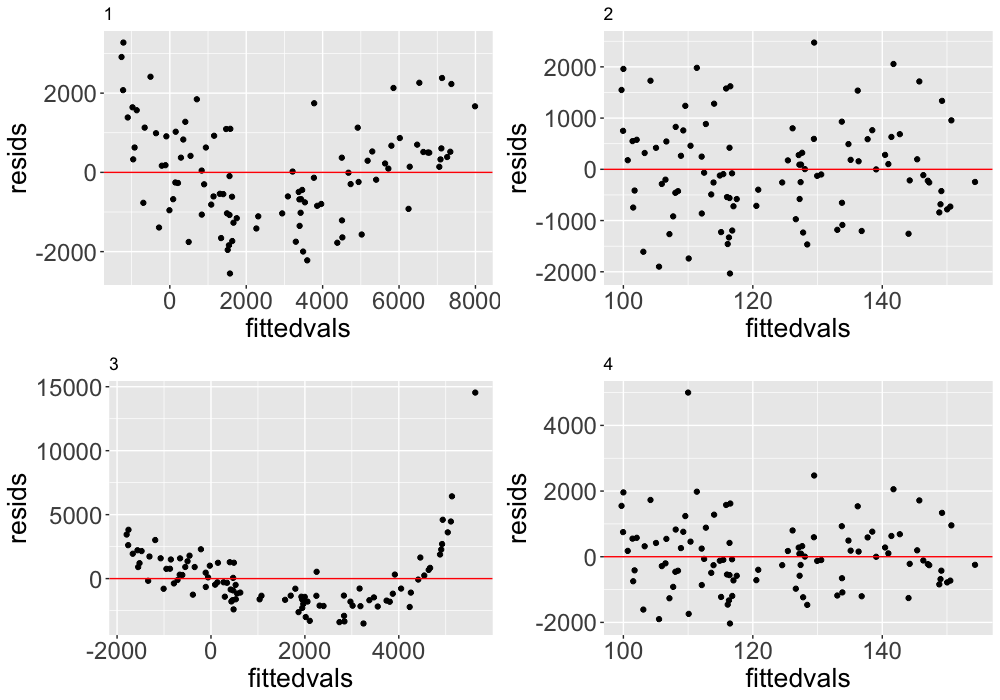
\includegraphics[scale=0.25]{lin_diagnostics_example.png}
%
%\end{frame}
%
%\begin{frame}{Linearity assumption: diagnostics}
%\textcolor{blue}{Question:} Do you think the linearity assumption is violated for models $1$ through $4$, based on the plots of fitted values vs. residuals?
%
%\vspace{0.3cm}
%
%\textcolor{blue}{Answer:} Models 1 and 3 both appear to violate the linearity assumption, but Models 2 and 4 appear okay (the assumption seemingly holds). 
%
%\vspace{0.3cm}
%
%\textbf{Diagnostic plots are not a perfect tool for assessing assumptions, and they are subject to (subjective) interpretation!} (this is true for all diagnostic plots covered in this chapter)
%\end{frame}
%
%% include a frame about what we can do if linearity is violated, or no???? ask Charlie
%
%\subsection{Independence}
%
%\begin{frame}{Independence assumption}
%\textcolor{blue}{Independence assumption:} The errors $\epsilon_i$, $i = 1, \dots, n$ are independent of each other.
%
%\vspace{0.3cm}
%
%What does it \textit{mean} for this assumption to be violated?
%
%\vspace{0.3cm}
%
%\begin{itemize}
%	\item[] Violating the independence assumption means that our observations are sampled in a way such that their responses are \textit{dependent}. Here are a few examples of when this might happen:
%	\begin{itemize}
%		\item We observe multiple individuals over time, and collect data on their outcomes at multiple time points. We expect the responses for a given individual to be \textit{dependent} over time (e.g. my weight tomorrow \textit{depends} on my weight today)
%		\item We collect standardized test scores from individuals in multiple schools. We expect students within the same to school (perhaps) to score similarly, as they've had similar educational experiences
%	\end{itemize}
%\end{itemize}
%\end{frame}
%
%\begin{frame}{Independence assumption: diagnostics}
%How do we assess whether or not the independence assumption is violated?
%
%\vspace{0.3cm}
%
%Think about how your data was collected! There are no diagnostic plots for this assumption.
%
%\vspace{0.3cm}
%
%\textcolor{blue}{Question:} For our births dataset, we have data from a random sample of birth parent's in King County. Do you think the independence assumption is violated for our simple linear regression example, with First Steps participation as the predictor and birthweight as the response? Why or why not? \pause
%
%\vspace{0.3cm}
%
%\textcolor{blue}{Answer:} The independence assumption is likely satisfied for this model. There is no reason to believe that the birthweight of a baby born to one birth parent would depend on the birthweight of a baby born to a different birth parent.
%
%\end{frame}
%
%\begin{frame}{Independence assumption: diagnostics}
%How do we assess whether or not the independence assumption is violated?
%
%\vspace{0.3cm}
%
%Think about how your data was collected! There are no diagnostic plots for this assumption.
%
%\vspace{0.3cm}
%
%\textcolor{blue}{Question:} Suppose instead we had information for all previous births for every individual in our dataset as well, so for each birth parent, there may be more than one of their births present in the dataset. Do you think the independence assumption is violated for a simple linear regression, with First Steps participation as the predictor and birthweight as the response? Why or why not? \pause
%
%\vspace{0.3cm}
%
%\textcolor{blue}{Answer:} The independence assumption is likely violated. It is reasonable to expect that the birthweight of a future child may be dependent on the birthweight of a past one. For example, it is known that having one premature birth puts you at increased risk for another premature birth in a future pregnancy, and babies born prematurely tend to have lower weights. 
%
%\end{frame}
%
%\subsection{Normality}
%
%\begin{frame}{Normality assumption}
%\textcolor{blue}{Normality assumption:} The errors $\epsilon_i$, $i = 1, \dots, n$ are normally distributed.
%
%\vspace{0.3cm}
%
%What does it \textit{mean} for this assumption to be violated?
%
%\vspace{0.3cm}
%
%\begin{itemize}
%	\item[] Violating the normality assumption means that our errors are not normally distributed. We like our errors to be normally distributed because our confidence intervals and hypothesis tests are based on the Normal or $t$ distribution, which assume underlying Normal data. \pause
%\end{itemize}
%
%\vspace{0.3cm} 
%\textcolor{red}{Question:} But what about the Central Limit Theorem? We know from the CLT that the sampling distribution of the sample mean is approximately normal in large samples\dots does the CLT also apply to regression coefficients?
%
%\end{frame}
%
%\begin{frame}{Normality assumption: do we need it?}
%
%\textcolor{blue}{Question:} Does the CLT also apply to regression coefficients, and what does this have to do with the normality assumption for linear regression?
%
%\vspace{0.3cm} 
%
%\textcolor{blue}{Answer:} The CLT \textit{does} apply to regression coefficients. The sampling distribution of a sample regression coefficient $\hat{\beta}$ is approximately normal \textcolor{red}{in large samples}, and is unbiased ($E[\hat{\beta}] = \beta$), \textbf{even if} the errors $\epsilon_i$ are not normally distributed! \pause
%
%\vspace{0.3cm} 
%
%\textcolor{blue}{Key Takeaway:} 
%\begin{itemize}
%	\item If our sample size is large, we do not need the normality assumption for linear regression because the Central Limit Theorem will kick in.
%	\item If our sample size is small, we do need the normality assumption for linear regression inference.
%\end{itemize}
%
%\small What sample size is considered ``large" enough? Many statistics courses / textbooks will say $n = 30$ or more is large enough for the CLT to kick in. 
%
%\end{frame}
%
%\begin{frame}{Normality assumption: diagnostics}
%In settings where we have a small sample size and need the normality assumption to hold, how do we assess whether not the normality assumption is violated?
%
%\vspace{0.3cm}
%
%We can make a histogram of \textcolor{blue}{residuals} to see if they look approximately normally distributed. If they look close to normal (a bell shaped curve), then the normality assumption is likely not violated.
%
%\vspace{0.3cm}
%
%\begin{itemize}
%	\item[] Reminder: a \textcolor{blue}{residual} is the difference between the observed value of the response variable $Y$ and the fitted value 
%\end{itemize}
%
%\vspace{0.3cm}
%
%\small You may also hear people refer to \textcolor{blue}{qq plots} for diagnosing the normality assumption, but we will not focus on those in this course (and you will not be tested on them)
%
%\end{frame}
%
%\begin{frame}[fragile]{Normality assumption: diagnostics in \texttt{R}}
%To plot make a histogram of residuals in \texttt{R}, we can use the following code for a given linear model object \texttt{mod}:
%
%\vspace{0.3cm}
%
%\begin{lstlisting}
%resids <- residuals(mod)
%data.frame(resids = resids) %>%
%    ggplot(aes(resids)) +
%    geom_histogram(bins = 10, col = "black")
%\end{lstlisting}
%
%\end{frame}
%
%\begin{frame}{Normality assumption: diagnostics in \texttt{R}}
%And we get plots that look something like this:
%
%	
%\begin{figure}
%	\centering 
%	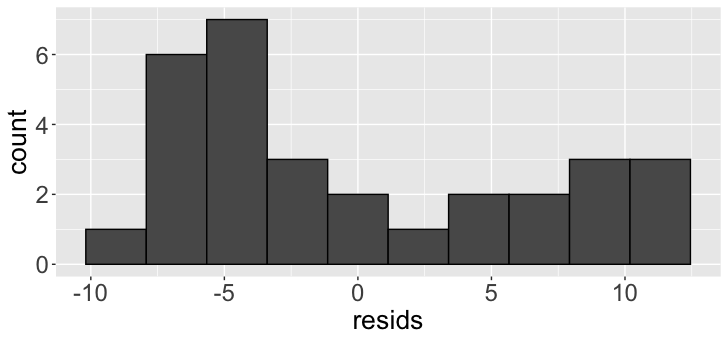
\includegraphics[scale=0.2]{hist_resid1.png} \\
%    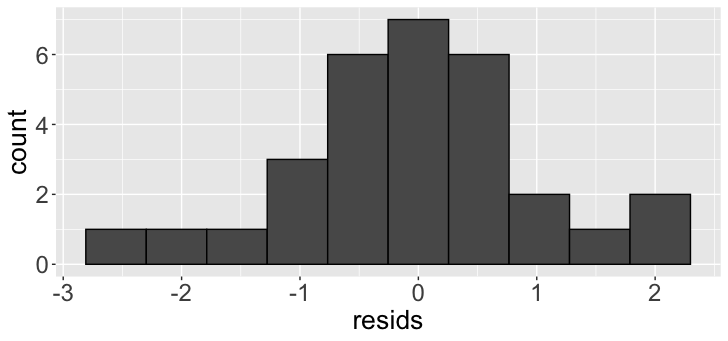
\includegraphics[scale=0.2]{hist_resid2.png}
%\end{figure}
%
%\textcolor{blue}{Question:} Do the residuals look close to normally distributed in either of these plots?
%
%\end{frame}
%
%\begin{frame}{Normality assumption: diagnostics in \texttt{R}}
%
%\textcolor{blue}{Question:} Do the residuals look close to normally distributed in either of these plots?
%
%\vspace{0.3cm}
%
%\textcolor{blue}{Answer:} The residuals in the lower plot seem to be approximately normally distributed, but not the residuals in the upper plot.
%
%\vspace{0.3cm}
%
%\textcolor{blue}{Note:} Diagnostic plots are not perfect, and it can be difficult to judge whether or not residuals look close ``enough" to normal state that the normally assumption is satisfied. This is one reason why having large sample sizes (and not needing to worry about this assumption) is so nice!
%
%\end{frame}
%
%\subsection{Equal variance}
%
%\begin{frame}{Equal variance assumption}
%\textcolor{blue}{Equal variance assumption:} The errors $\epsilon_i$, $i = 1, \dots, n$ all have the same variance.
%
%\vspace{0.3cm}
%
%What does it \textit{mean} for this assumption to be violated?
%
%\begin{itemize}
%	\item[] Violating the equal variance assumption means that in reality, our errors have different variances. This assumption is often easier to visualize graphically (which we do on the next slide)
%\end{itemize}
%
%\end{frame}
%
%\begin{frame}{Equal variance assumption}
%
%The top plot shows an example of constant variance, and the bottom an example of nonconstant variance:
%
%\vspace{0.3cm}
%
%\centering
%
%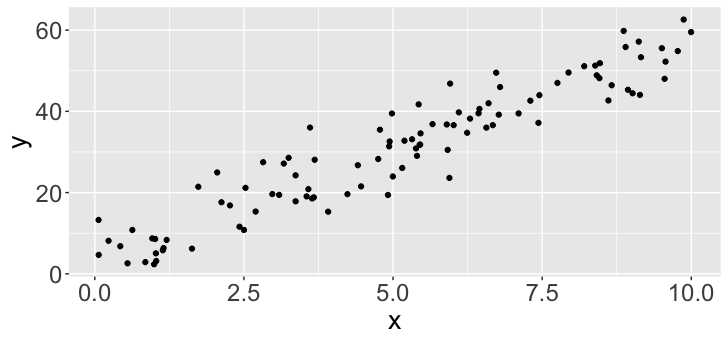
\includegraphics[scale=0.2]{constvar.png}
%
%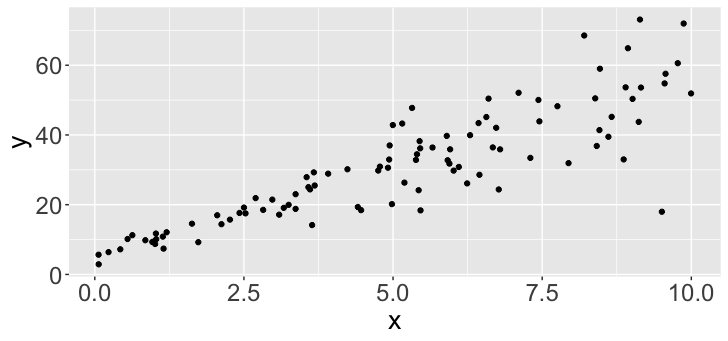
\includegraphics[scale=0.2]{nonconstvar.png}
%
%\end{frame}
%
%\begin{frame}{Equal variance assumption}
%How can we tell by looking at a scatterplot of our outcome ($y$) vs. our predictor ($x$)?
%
%\vspace{0.3cm}
%
%If our errors $\epsilon_i$ have equal variance, the spread of the $y$ values should be equal, across all values of $x$.
%% draw here on ipad
%
%\vspace{0.3cm}
%\centering
%
%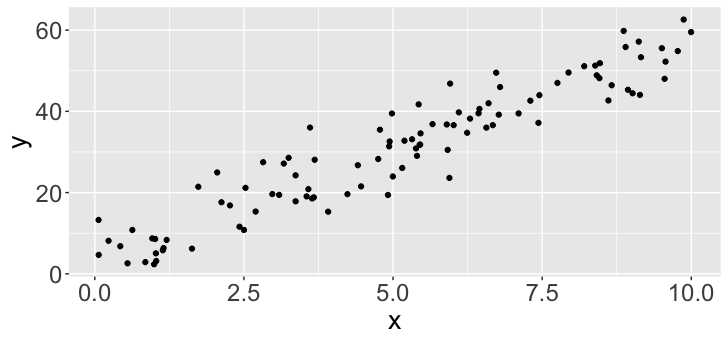
\includegraphics[scale=0.3]{constvar.png}
%
%\end{frame}
%
%\begin{frame}{Equal variance assumption}
%How can we tell by looking at a scatterplot of our outcome ($y$) vs. our predictor ($x$)?
%
%\vspace{0.3cm}
%
%If our errors $\epsilon_i$ have \textit{unequal} variance, the spread of the $y$ values should be \textit{unequal}, across values of $x$.
%
%\vspace{0.3cm}
%% draw here on ipad
%\centering
%
%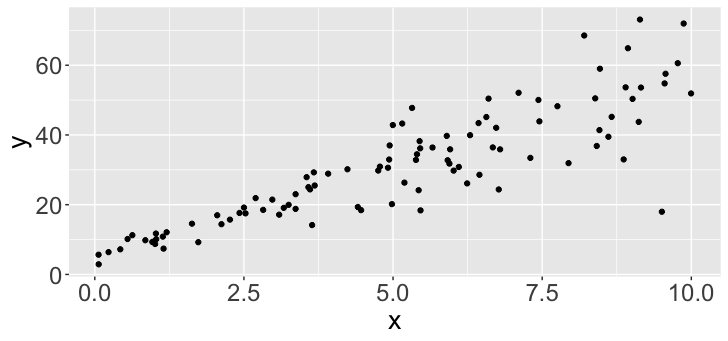
\includegraphics[scale=0.3]{nonconstvar.png}
%
%\end{frame}
%
%\begin{frame}{Equal variance assumption: diagnostics}
%Looking at scatterplots is useful, but how do we more clearly assess whether or not the equal variance assumption is violated?
%
%\vspace{0.3cm}
%
%We can plot \textcolor{blue}{residuals} vs. \textcolor{blue}{fitted values} using our linear regression output, and diagnose the assumption based on a scatter plot comparing the two.
%
%\vspace{0.3cm}
%
%Note that this is the same diagnostic plot we use to assess the linearity assumption, but we look for something slightly different:
%
%\vspace{0.3cm}
%
%\begin{itemize}
%	\item Linearity: assumption holds if residuals fall in a straight line at $y = 0$
%	\item Equal variance: assumption holds if residuals have a roughly even spread above and below the line $y = 0$ across different fitted values
%\end{itemize}
%
%\end{frame}
%
%
%\begin{frame}{Equal variance assumption: diagnostics in \texttt{R}}
%The code for plotting residuals vs. fitted values in \texttt{R} is the same as for the linearity assumption (since it's the same plot!). Our residual plots then look like\dots
%
%\centering
%
%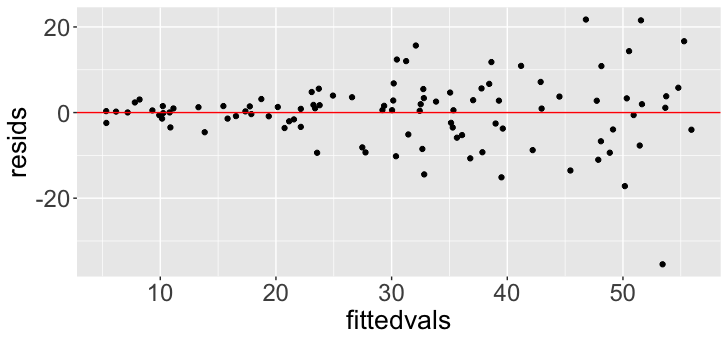
\includegraphics[scale=0.2]{eqvar_resids1.png}
%
%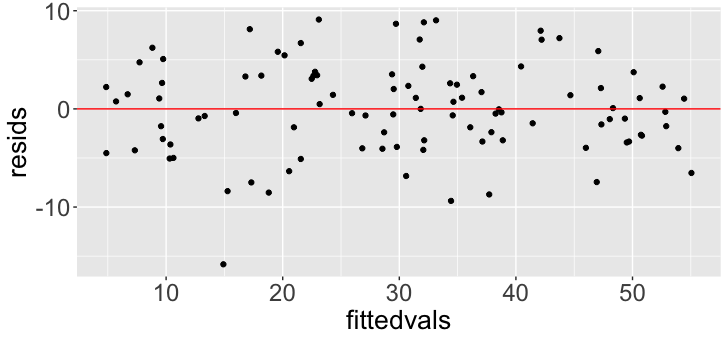
\includegraphics[scale=0.2]{eqvar_resids2.png} \pause
%
%\textcolor{blue}{Question:} Do you think the equal variance assumption holds for either of the models that generated these diagnostic plots?
%
%\end{frame}
%
%\begin{frame}{Equal variance assumption: diagnostics}
%\textcolor{blue}{Question:} Do you think the equal variance assumption holds for either of the models that generated these diagnostic plots?
%
%\vspace{0.3cm}
%
%\textcolor{blue}{Answer:} The equal variance assumption seems to hold for the bottom plot, but not the top plot. The spread of residuals around the line $y = 0$ is much wider for larger fitted values in the top plot. 
%\end{frame}
%
%\begin{frame}{Equal variance assumption: do we need it?}
%We previously mentioned that we may not always need the equal variance assumption for linear regression:
%
%\vspace{0.3cm}
%
%\begin{itemize}
%	\item Assumption needed: when using \textbf{naive} standard errors 
%	\item Assumption not needed: when using \textbf{robust} standard errors
%\end{itemize}
%
%\vspace{0.3cm}
%
%Naive standard errors are what we've used so far in the course, and will continue to use throughout (this is what the \texttt{lm} function in \texttt{R} returns by default). Robust standard errors are a statistical tool that allow us to relax the assumption of equal variance. \textit{We will not be going into detail in this course on robust standard errors.}
%
%\vspace{0.3cm}
%
%\small \textcolor{blue}{What you need to know:} For everything we do in this course, we are using \textit{naive} standard errors, and so we need the equal variance assumption to hold. More advanced statistical tools exist (specifically, robust standard errors) that can allow us to relax this assumption, even though we won't be using them in this course.
%
%\end{frame}
%
%\begin{frame}{Linear regression assumptions: Recap}
%The \textit{classical} linear regression (\textcolor{red}{LINE}) assumptions are:
%
%\vspace{0.3cm}
%
%\begin{itemize}
%	\item \textcolor{red}{L}inearity: There is a linear relationship between $X_i$ and the true population conditional mean $Y_i \mid X_i$
%	\item \textcolor{red}{I}ndependence: The errors are independent of each other
%	\item \textcolor{red}{N}ormality: The errors are normally distributed
%	\item \textcolor{red}{E}qual variance: The errors have the same variance
%\end{itemize} \pause
%
%\vspace{0.3cm}
%
%Diagnostics for each of these assumptions are:
%
%\vspace{0.3cm}
%
%\begin{itemize}
%	\item \textcolor{red}{L}inearity: Scatterplot of fitted values vs. residuals
%	\item \textcolor{red}{I}ndependence: Think about the data collection!
%	\item \textcolor{red}{N}ormality: Histogram of residuals
%	\item \textcolor{red}{E}qual variance: Scatterplot of fitted values vs. residuals
%\end{itemize}
%
%\end{frame}
%
%\begin{frame}{Linear regression assumptions: Recap}
%The \textit{classical} linear regression (\textcolor{red}{LINE}) assumptions are:
%
%\vspace{0.3cm}
%
%\begin{itemize}
%	\item \textcolor{red}{L}inearity: There is a linear relationship between $X_i$ and the true population conditional mean $Y_i \mid X_i$
%	\item \textcolor{red}{I}ndependence: The errors are independent of each other
%	\item \textcolor{red}{N}ormality: The errors are normally distributed
%	\item \textcolor{red}{E}qual variance: The errors have the same variance
%\end{itemize}
%
%\vspace{0.3cm}
%
%The assumptions we need (in this course) when we have \textit{large} samples are:
%
%\vspace{0.3cm}
%
%\begin{itemize}
%	\item \textcolor{red}{L}inearity
%	\item \textcolor{red}{I}ndependence
%	\item \sout{\textcolor{red}{N}ormality}
%	\item \textcolor{red}{E}qual variance
%\end{itemize}
%
%\end{frame}
%
%\begin{frame}{Linear regression assumptions: Recap}
%The \textit{classical} linear regression (\textcolor{red}{LINE}) assumptions are:
%
%\vspace{0.3cm}
%
%\begin{itemize}
%	\item \textcolor{red}{L}inearity: There is a linear relationship between $X_i$ and the true population conditional mean $Y_i \mid X_i$
%	\item \textcolor{red}{I}ndependence: The errors are independent of each other
%	\item \textcolor{red}{N}ormality: The errors are normally distributed
%	\item \textcolor{red}{E}qual variance: The errors have the same variance
%\end{itemize}
%
%\vspace{0.3cm}
%
%The assumptions we need when we have \textit{large} samples and use \textit{robust standard errors}:
%
%\vspace{0.3cm}
%
%\begin{itemize}
%	\item \textcolor{red}{L}inearity
%	\item \textcolor{red}{I}ndependence
%	\item \sout{\textcolor{red}{N}ormality}
%	\item \sout{\textcolor{red}{E}qual variance}
%\end{itemize}
%
%\end{frame}


%\section{Transformations}
%
%\begin{frame}{Interpreting coefficients (no transformation)}
%In the previous section we learned how to interpret $\beta_0$ and $\beta_1$ in a linear regression model:
%
%$$
%E[Y \mid X] = \beta_0 + \beta_1 X
%$$
%
%\vspace{0.2cm}
%
%$\beta_0$ is the mean value of $Y$ among subjects with $X = 0$
%
%\vspace{0.3cm}
%
%$\beta_1$ is the difference in mean value of $Y$ comparing two groups that differ by one unit in $X$
%
%
%\end{frame}
%
%\begin{frame}{Interpreting coefficients (no transformation)}
%In the previous section we learned how to interpret $\beta_0$ and $\beta_1$ in a linear regression model \textcolor{blue}{in context}:
%
%$$
%E[\text{bwt} \mid \text{age}] = \beta_0 + \beta_1 \times \text{age}
%$$
%
%\vspace{0.2cm}
%
%$\beta_0$ is the mean value of $Y$ among subjects with $X = 0$
%
%\begin{itemize}
%	\item[] \textcolor{blue}{mean birthweight (grams) of babies born to birth parents of age zero}
%\end{itemize}
%
%
%\vspace{0.3cm}
%
%$\beta_1$ is the difference in mean value of $Y$ comparing two groups that differ by one unit in $X$
%
%\begin{itemize}
%	\item[] \textcolor{blue}{difference in mean birthweight (grams) comparing two groups of birth parents that differ by one year in age}
%\end{itemize} 
%
%\end{frame}
%
%\begin{frame}{Interpreting coefficients after a transformation}
%How do we interpret $\beta_0$ in this linear regression model?
%
%$$
%E[\text{bwt} \mid \textcolor{blue}{(\text{age} - 25)}] = \beta_0 + \beta_1 \times \textcolor{blue}{(\text{age} - 25)}
%$$
%
%\vspace{0.2cm}
%
%$\beta_0$ is the mean value of $Y$ among subjects with $X = 0$
%\pause
%\begin{itemize}
%	\item[] mean birthweight (grams) of babies born to birth parents with $\text{age} - 25 = 0$ \pause
%	\item[] \textcolor{blue}{mean birthweight (grams) of babies born to 25 yr. old birth parents } \pause
%\end{itemize} 
%
%\vspace{0.3cm}
%
%Why are those last two interpretations equivalent?
%\begin{align*}
%\text{age} - 25 &= 0 \\
%\text{age} & = 25
%\end{align*}
%
%\end{frame}
%
%\begin{frame}{Interpreting coefficients after a transformation}
%How do we interpret $\beta_1$ in this linear regression model?
%
%$$
%E[\text{bwt} \mid \textcolor{blue}{(\text{age} - 25)}] = \beta_0 + \beta_1 \times \textcolor{blue}{(\text{age} - 25)}
%$$
%
%\vspace{0.2cm}
%
%$\beta_1$ is the difference in mean value of $Y$ comparing two groups that differ by one unit in $X$
%
%\begin{itemize}
%	\item[] difference in mean birthweight (grams) comparing two groups of birth parents that differ in (age - 3) by one year
%	\item[] \textcolor{blue}{difference in mean birthweight (grams) comparing two groups of birth parents that differ in age by one year}
%\end{itemize} 
%
%\vspace{0.3cm}
%
%Why are those last two interpretations equivalent?
%\begin{align*}
%\text{age} - 25 = x + 1 \hspace{0.1cm}& \textcolor{red}{vs}  \hspace{0.1cm}\text{age} - 25 = x \\
%\text{age} = x + 26 \hspace{0.1cm}& \textcolor{red}{vs}  \hspace{0.1cm}\text{age}  = x + 25
%\end{align*}
%
%\end{frame}
%
%\begin{frame}{Transformations: Practice}
%With a partner\dots
%
%\vspace{0.3cm}
%
%\begin{enumerate}
%	\item Interpret $\beta_0, \beta_1$ in the following models:
%	\begin{enumerate}
%		\item $E[\text{bwt} \mid \text{age}] = \beta_0 + \beta_1 (\text{age} - \bar{\text{age}})$
%		\item $E[\text{bwt} \mid \text{age}] = \beta_0 + \beta_1 \left( \frac{\text{age}}{5} \right)$
%		\item $E[\text{bwt} \mid \text{age}] = \beta_0 + \beta_1 \left( \frac{\text{age} - 25}{5} \right)$
%	\end{enumerate}
%\item[]
%	\item Interpret $\beta_0, \beta_1$ in the following models:
%	\begin{enumerate}
%		\item $E[(\text{bwt} \times 50) \mid \text{age}] = \beta_0 + \beta_1 (\text{age})$
%		\item $E[(\frac{\text{bwt}}{453.592}) \mid \text{age}] = \beta_0 + \beta_1 (\text{age})$
%		\item[] \tiny (Hint: 1 pound = 453.592 grams)
%	\end{enumerate}
%\end{enumerate}
%
%% give them 15 minutes (?) to work, then discuss as a class
%
%\end{frame}
%
%\subsection{Linear transformations of $X$ and $Y$}
%
%\begin{frame}{Linear transformations of $X$ and $Y$}
%\textcolor{blue}{Linear transformations:} adding, subtracting, multiplying, and/or dividing by some constant
%
%\vspace{0.3cm}
%
%Which transformations change the interpretation of $\beta_0$? \pause
%\begin{itemize}
%	\item[] Adding (subtracting) a constant to (from) $X$
%	\item[] Any change to $Y$ 
%\end{itemize} \pause
%
%\vspace{0.3cm}
%
%Which transformations change the interpretation of $\beta_1$? \pause
%\begin{itemize}
%	\item[] Multiplying (dividing) $X$ by a constant
%	\item[] Multiplying (dividing) $Y$ by a constant 
%\end{itemize}
%\end{frame}
%
%\begin{frame}{Why transform $X$ and/or $Y$?}
%Why might we want to transform our variables?
%
%\begin{itemize}
%	\item Transforming can \textit{make our interpretation of} $\beta_0$ \textit{more scientifically meaningful} (e.g., so we're not talking about the average birthweight of a baby born to a 0 yr. old birth parent)
%	\item Transforming can \textit{change the units of the outcome and/or predictor} (e.g., difference in birthweight in pounds vs. grams, comparing two groups that differ by one year in age)
%\end{itemize}
%\end{frame}
%
%\subsection{Log transformations of $X$ and $Y$}
%
%\begin{frame}{Log transformations: $\beta_0$ interpretation}
%So far we've seen linear transformations. What about log transformations? Consider the model
%$$
%E[\text{bwt} \mid \text{wpre}] = \beta_0 + \beta_1 \log(\text{wpre})
%$$
%where wpre = birth parent's pre-pregnancy weight in pounds.
%
%\vspace{0.3cm}
%
%$\beta_0$ is the mean value of $Y$ among subjects with $X = 0$
%
%\vspace{0.3cm}
%
%\tiny *Note: in statistics (and in \texttt{R}) when we write log, we mean $\text{log}_e = \text{ln}$. If we are using a different base, we'll explicitly write it
%
%\end{frame}
%
%\begin{frame}{Log transformations: $\beta_0$ interpretation}
%So far we've seen linear transformations. What about log transformations? Consider the model
%$$
%E[\text{bwt} \mid \text{wpre}] = \beta_0 + \beta_1 \log(\text{wpre})
%$$
%where wpre = birth parent's pre-pregnancy weight in pounds.
%
%\vspace{0.3cm}
%
%$\beta_0$ is the mean value of $Y$ among subjects with $X = 0$
%
%\begin{itemize}
%	\item[] mean birthweight (grams) of babies born to birth parents with log(wpre) = 0\pause
%	\item[] \textcolor{blue}{mean birthweight (grams) of babies born to birth parents with a pre-pregnancy weight of 1 pound}
%\end{itemize}
%
%\end{frame}
%
%\begin{frame}{Log transformations: $\beta_0$ interpretation}
%
%$\beta_0$ is the mean value of $Y$ among subjects with $X = 0$
%
%\begin{itemize}
%	\item[] mean birthweight (grams) of babies born to birth parents with log(wpre) = 0
%	\item[] \textcolor{blue}{mean birthweight (grams) of babies born to birth parents with a pre-pregnancy weight of 1 pound}
%\end{itemize}
%
%\vspace{0.3cm}
%
%
%Why are those last two interpretations equivalent?
%
%
%\begin{align*}
%\log(\text{wpre}) & = 0 \\
%e^{\log(\text{wpre})} & = e^0 \\
%\text{wpre} & = 1
%\end{align*}
%
%\end{frame}
%
%
%\begin{frame}{Log transformations: $\beta_1$ interpretation}
%
%$\beta_1$ is the difference in mean value of $Y$ comparing two groups that differ by one unit in $X$\pause
%
%\begin{itemize}
%	\item[] difference in mean birthweight (grams) comparing two groups of birth parents that differ in $\log(\text{wpre})$ by one unit \pause
%	\item[] \textcolor{blue}{difference in mean birthweight (grams) comparing two groups of birth parents that differ in pre-pregnancy weight by a multiplicative factor of $e$ (2.718\dots)}
%\end{itemize} \pause
%
%\vspace{0.3cm}
%
%
%Why are those last two interpretations equivalent?
%
%
%\begin{align*}
%\log(\text{wpre})  = x + 1 \hspace{0.1cm} & \textcolor{red}{vs} \hspace{0.1cm} \log(\text{wpre})  = x  \\
%e^{\log(\text{wpre})}  = e^{x + 1}  \hspace{0.1cm} & \textcolor{red}{vs} \hspace{0.1cm} e^{\log(\text{wpre})}  = e^{x}\\
%\text{wpre}  = e^x e \hspace{0.1cm} & \textcolor{red}{vs} \hspace{0.1cm} \text{wpre} = e^x
%\end{align*}
%
%\end{frame}
%
%\begin{frame}{Log transformations: $\beta_1$ interpretation}
%An $e$-fold difference between two groups is not particularly intuitive.
%
%How can we make our interpretation of $\beta_1$ more intuitive?
%
%\vspace{0.3cm}
%
%Option 1: use a different base\pause
%
%\begin{itemize}
%	\item $E[\text{bwt} \mid \text{wpre}] = \beta_0 + \beta_1 \textcolor{blue}{\text{log}}_2 (\text{wpre})$
%	\begin{itemize}
%		\item $\beta_0$: mean birthweight among babies born to birth parents with pre-pregnancy weight of 1 pound
%		\item $\beta_1$: difference in mean birthweight comparing groups of birth parents that differ in pre-pregnancy weight by a \textcolor{blue}{multiplicative factor of 2}
%	\end{itemize} \pause
%\item $E[\text{bwt} \mid \text{wpre}] = \beta_0 + \beta_1 \textcolor{blue}{\text{log}}_{10} (\text{wpre})$
%\begin{itemize}
%	\item $\beta_0$: mean birthweight among babies born to birth parents with pre-pregnancy weight of 1 pound
%	\item $\beta_1$: difference in mean birthweight comparing groups of birth parents that differ in pre-pregnancy weight by a \textcolor{blue}{multiplicative factor of 10}
%\end{itemize} 
%\end{itemize}
%\end{frame}
%
%\begin{frame}{Log transformations: $\beta_1$ interpretation}
%An $e$-fold difference between two groups is not particularly intuitive.
%
%How can we make our interpretation of $\beta_1$ more intuitive?
%
%\vspace{0.3cm}
%
%Option 2: fit the same model but interpret $c \times \beta_1$ rather than $\beta_1$\pause
%
%\vspace{0.3cm}
%
%\textit{Example}: $\textcolor{blue}{\text{log}(1.1)}\beta_1$ is the difference in average birthweight comparing two groups of birth parents that differ in pre-pregnancy weight by a \textcolor{blue}{multiplicative factor of 1.1} (i.e. a 10\% difference)\pause
%
%
\includegraphics[scale=0.01]{chilipepper.png}
%\begin{align*}
%E[\text{bwt} \mid & \log(\text{wpre} = 1.1x)] - E[\text{bwt} \mid \log(\text{wpre} = x)] \\
%& = [\beta_0 + \beta_1 \log(1.1x)] - [\beta_0 + \beta_1 \log(x)] \\
%& = \beta_1 \log(1.1x) - \beta_1 \log(x) \\
%& = \beta_1 (\log(1.1) + \log(x)) - \beta_1 \log(x) \\
%& = \beta_1 \log(1.1)
%\end{align*}
%
%\end{frame}
%
%\begin{frame}{Log transformations: recap}
%Tying it all together\dots
%
%\vspace{0.3cm}
%
%\begin{itemize}
%	\item \textcolor{blue}{Regression model:} $E[\text{bwt} \mid X] = \beta_0 + \beta_1 \log(X)$
%	\item \color{blue} $\beta_0$\color{black}: average value of $Y$ among subjects with $X = 1$
%	\item \color{blue}$\log(k) \times \beta_1$\color{black}: difference in average value of $Y$ comparing two groups that differ in $X$ by a multiplicative factor of $k$
%\end{itemize}\pause
%
%\vspace{0.3cm}
%
%Why would we want to do this type of transformation?
%
%\begin{itemize}
%	\item Sometimes it is more scientifically relevant to talk about \textit{multiplicative changes} in $X$ rather than \textit{differences} in $X$
%	\item Types of variables that are often log transformed:
%	\begin{itemize}
%		\item Money (e.g., salary, GDP)
%		\item Biological measurements (e.g., prostate specific antigen in prostate cancer, serum creatinine in kindey disease)
%	\end{itemize}
%\end{itemize}
%\end{frame}
%
%\begin{frame}
%\frametitle{Transformations: $\log(Y)$}
%\begin{center} $E[\log(\text{bwt}) \mid \text{age}] = \beta_0 + \beta_1 \times age$ \end{center}
%$\beta_0$: average value of $Y$ among subjects with $X = 0$\\ \pause
%\begin{itemize}
%	\item[] average log birthweight babies born to 0 yr. old birth parents  \pause
%	\item[] log geometric mean birthweight among babies born to 0 yr. old birth parents \pause
%\end{itemize}
%\color{blue} $e^{\beta_0}$: geometric mean birthweight among babies born to 0 yr. old birth parents \color{black}\pause
%\vspace{0.3cm}
%
%Why are those interpretations equivalent?
%\begin{itemize}
%	\item[] \textit{Arithmetic mean}: $\frac{1}{n} \sum_{i=1}^n a_i$
%	\item[] \textit{Geometric mean}: $\left(\prod_{i=1}^n a_i\right)^{\frac{1}{n}} = e^{\frac{1}{n} \sum_{i=1}^n \log(a_i)}$
%\end{itemize}
%
%\vspace{0.3cm}
%
%\begin{footnotesize}The \color{blue} ``average of $\log(Y)$" \color{black} = $\frac{1}{n}\sum \log(Y_i)$ \ \color{blue} \textit{is the same as} \color{black}\\the \color{blue}``log of the geometric mean of $Y$" \color{black}= $\log(e^{\frac{1}{n}\sum \log(Y_i)} = \frac{1}{n}\sum \log(Y_i)$.\end{footnotesize}
%\end{frame}
%
%\begin{frame}
%\frametitle{Transformations: $\log(Y)$}
%\begin{center} $E[\log(\text{bwt})\mid \text{age}] = \beta_0 + \beta_1 \text{age}$ \end{center}
%$\beta_1$: difference in average values of $Y$ comparing two groups that differ in $X$ by one unit\\ \pause
%\begin{itemize}
%	\item[] difference in average $\log(\text{bwt})$ comparing two ...\pause
%	\item[] difference in log geometric mean birthweight comparing two ... \pause
%\end{itemize}
%\color{blue} $e^{\beta_1}$: ratio of geometric mean birthweight comparing two ... \color{black} \pause
%\vspace{0.3cm}
%
%Why are those interpretations equivalent?
%
%
\includegraphics[scale=0.01]{chilipepper.png}
%\begin{align*}
%\beta_1 & = \log(\text{GM}[Y|X=x+1])-\log(\text{GM}[Y|X=x])\\
%& = \log\left(\text{GM}[Y|X=x+1]\div\text{GM}[Y|X=x]\right)\\
%e^{\beta_1} & = \text{GM}[Y|X=x+1]\div\text{GM}[Y|X=x]
%\end{align*}
%\end{frame}
%
%\begin{frame}{Transformations: log(Y) recap}
%Tying it all together\dots
%
%\vspace{0.3cm}
%
%\begin{itemize}
%	\item \textcolor{blue}{Regression model:} $E[\log(\text{bwt}) \mid X] = \beta_0 + \beta_1 \log(X)$
%	\item \color{blue} $e^{\beta_0}$\color{black}: geometric mean of $Y$ among subjects with $X = 0$
%	\item \color{blue}$e^{\beta_1}$\color{black}: ratio of geometric means of $Y$ comparing two groups that differ in $X$ by one unit
%\end{itemize} \pause
%
%\vspace{0.3cm}
%
%Why would we want to do this type of transformation?
%
%\begin{itemize}
%	\item Sometimes it is more scientifically relevant to talk about \textit{multiplicative changes} in $X$ rather than \textit{differences} in $X$
%	\item Types of variables that are often log transformed:
%	\begin{itemize}
%		\item Money (e.g., salary, GDP)
%		\item Biological measurements (e.g., prostate specific antigen in prostate cancer, serum creatinine in kindey disease)
%	\end{itemize}
%\end{itemize}
%\begin{footnotesize}
%	Practitioners often log transform highly skewed variables in order to move the data closer to a Normal distribution. In large sample sizes, though, we do not need Normality. 
%\end{footnotesize}
%\end{frame}
%
%% hw question maybe where we have both x and y log transformed
%\begin{frame}
%\frametitle{Transformations: polynomial}
%Another common transformation is the quadratic transformation\dots
%\begin{center} $E[\text{bwt} \mid \text{age}] = \beta_0 + \beta_1 \times \text{age} + \beta_2 \times \text{age}^2$ \end{center}
%
%Now we have three coefficients: $\beta_0, \beta_1, \beta_2$\pause
%
%\vspace{0.3cm}
%
%\color{blue} $\beta_0$: average birthweight among babies born to birth parents who are 0 yrs. old \color{black} \pause
%\begin{align*}
%E[\text{bwt} \mid \text{age} = 0] & = \beta_0 + \beta_1 (0) + \beta_2(0)^2 \\
%& = \beta_0 + 0 + 0 \\
%& = \beta_0
%\end{align*}
%\end{frame}
%
%\begin{frame}
%\frametitle{Transformations: polynomial}
%Another common transformation is the quadratic transformation\dots
%\begin{center} $E[\text{bwt} \mid \text{age}] = \beta_0 + \beta_1 \times \text{age} + \beta_2 \times \text{age}^2$ \end{center}
%
%$\beta_1$: \color{red} NOT \color{black} the difference in average birthweight comparing groups of birth parents that differ in age by one year \pause
%\begin{align*}
%E[& \text{bwt} \mid \text{age} = x + 1] -E[\text{bwt} \mid \text{age} = x]\\
%& = \left[\beta_0 + \beta_1 (x+1) + \beta_2(x+1)^2\right] -\left[\beta_0 + \beta_1 (x) + \beta_2(x)^2\right]\\
%& = \beta_1 + \beta_2(2x+1) \\
%\end{align*}\pause
%\color{blue} $\beta_1,\beta_2$: no straightforward interpretation \color{black}
%\end{frame}
%
%\begin{frame}
%\frametitle{Transformations: polynomial recap}
%Tying it all together...
%\begin{itemize}
%	\item \color{blue} Regression model: \color{black} $E[Y|X] = \beta_0 + \beta_1X + \beta_2 X^2 + \cdots$
%	\item \color{blue} $\beta_0$: \color{black} average value of $Y$ when $X = 0$
%	\item \color{blue} $\beta_1, \beta_2, \cdots$: \color{black} no straightforward interpretation
%\end{itemize}\pause
%
%\vspace{0.3cm}
%
%Why would we want to do this type of transformation?
%\begin{itemize}
%	\item Sometimes we might have scientific reason to believe that $Y$ is related to $X^2$ (e.g., area) or $X^3$, rather than just $X$
%	\item Model non-linearity in the relationship between $X$ and $Y$
%	\begin{itemize}
%		\item May be important for prediction (we'll return to this later)
%		\item Not necessary for showing associations 
%	\end{itemize}
%\end{itemize}
%
%\vspace{0.3cm}
%
%Real world example:  \href{https://www.ncbi.nlm.nih.gov/pmc/articles/PMC4046865/}{\color{cyan} the log-quad model for mortality estimation}
%
%\end{frame}
%
%\begin{frame}
%\frametitle{Summary: why transform $X$ and/or $Y$?}
%Why might we want to transform our variables? \vspace{0.3cm}
%\begin{itemize}
%	\item Scientific motivation
%	\begin{itemize}
%		\item Improve interpretation
%		\item More realistically model the relationships we think exist between variables
%		\begin{itemize}
%			\item Multiplicative (ratio) vs additive (difference)
%			\item Geometric mean vs arithmetic mean
%		\end{itemize}
%	\end{itemize}
%	\item Account for non-linearity 
%	\begin{itemize}
%		\item Important for prediction
%		\item Not necessarily for detecting associations
%	\end{itemize}
%\end{itemize}
%\end{frame}
%
%\begin{frame}[c]
%\centering \huge Any Questions?
%\end{frame}

\end{document}